%%%%%%%%%%
% Header %
%%%%%%%%%%
%\documentclass[12pt, preprint]{aastex}
%\documentclass[onecolumn]{emulateapj}
\documentclass{emulateapj}
\usepackage{apjfonts}
\usepackage{graphicx}
\usepackage{here,lscape}
\shorttitle{X-ray Band Dependent Temperature}
\shortauthors{Cavagnolo et al.}
\bibliographystyle{apj}
\newcommand{\tf}{T$_{HFR}$ }
\newcommand{\hard}{T$_{2.0_{\text{rest}}-7.0}$ }
\newcommand{\full}{T$_{0.7-7.0}$ }

%%%%%%%%%%%%%%%%%%%%%
% Title and Authors %
%%%%%%%%%%%%%%%%%%%%%

\begin{document}
\title{X-ray Band Dependence of Best-Fit \\
	Temperature in Galaxy Clusters}
\author{Kenneth W. Cavagnolo\altaffilmark{1,2}, Megan
Donahue\altaffilmark{1}, G. Mark Voit\altaffilmark{1}, and Ming
Sun\altaffilmark{1}}
\altaffiltext{1}{Department of Physics and Astronomy, Michigan State
University, BPS Building, East Lansing, MI 48824}
\altaffiltext{2}{cavagnolo@pa.msu.edu}

%%%%%%%%%%%%
% Abstract %
%%%%%%%%%%%%

\begin{abstract}
We present a study of energy band dependance on best-fit temperatures
for a sample of 154 clusters of galaxies selected from the Chandra
Data Archive. \cite{2001ApJ...546..100M} found simulated clusters far from
virialization were much cooler than the cluster mass-observable
scaling relations predict; motivated by this work, we perform an
observational analog to test their predictions. We measure
temperatures for our sample clusters in apertures of R$_{5000}$ and
R$_{2500}$ in a full energy band, 0.7-7.0 keV, and a hard energy band,
2.0$_{\text{rest}}$-7.0 keV. We measure a clear departure from unity of the
ratio T$_{\text{hard}}$/T$_{\text{full}}$ (\tf) at $> 6\sigma$. We also find
increasing values of \tf favor non-cool core clusters over cool-core
clusters. In addition, clusters with the largest values of \tf are all
mergers without cool cores. We propose \tf may be used as an additional metric in
measuring the departure of simulated clusters from expected scaling
relations. \tf, along with other metrics such as power ratio and
measures of substructure, might prove useful in reducing the scatter,
and hence uncertainty, in relations such as mass-temperature and
mass-luminosity which are essential in cosmological studies.
\end{abstract}

%%%%%%%%%%%%
% Keywords %
%%%%%%%%%%%%

\keywords{catalogs -- galaxies: clusters: general -- X-rays:
  galaxies: clusters -- cosmology: observations -- methods: data
  analysis}

%%%%%%%%%%%%%%%%%%%%%%%%%%%%%%%%%%%%%%%
\section{Introduction}\label{sec:intro}
%%%%%%%%%%%%%%%%%%%%%%%%%%%%%%%%%%%%%%%

With the discovery of dark energy, clusters of galaxies have entered
a renaissance for their utility in cosmology studies. Cluster number
counts as a function of redshift, $dN/dz$, specifically for clusters above a
given mass threshold, has been proposed as a highly
sensitive observational tool for measuring cosmological parameters
\citep{1989ApJ...341L..71E, 1998ApJ...508..483W, 2001ApJ...553..545H,
2003PhRvD..67h1304H, 2004PhRvD..70l3008W}.
However, cluster counts are only a useful
cosmological tool if we can understand the cluster mass function
statistically. Unlike simple gravitational systems where mass can be
directly measured from the behavior of objects residing within
the potential well, clusters are a complex system of merging galaxies
and a much more massive gaseous component, the intracluster medium (ICM).
The ICM records the hierarchical formation history of a cluster and
given the proper conditions will come into hydrostatic equilibrium
within the cluster potential
\citep{2005RvMP...77..207V,1996ApJ...469..494E}. The ICM X-ray
properties of temperature and density can then be used to infer the
mass of a cluster using the equation of hydrostatic equilibrium.

However, idealizing clusters as being in hydrostatic equilibrium is
the exception and not the rule. The signature of pure gravitational
construction of a cluster is altered by a continuum of merger
activity, feedback mechanisms such as AGN, and prodigious radiative
cooling on time scales shorter than a Hubble time. To better
understand the cluster mass function, and consequently dark energy, we
must find methods for increasing the accuracy and predicitve power of the statistical
mass-observable scaling relations which are currently the largest
source of uncertainty in studies of $dN/dz$, {\textit{in addition}} to
quantifying the intrinsic scatter within these relations created by
cluster substructure \citep{2005PhRvD..72d3006L}.

To these ends, we must understand the dynamical state of a cluster
beyond the binary descriptor of ``hydrostatic equilibrium equals yes
or no.'' The answer for all clusters is that they exist in a dynamical
state somewhere in the middle \citep{2006ApJ...639...64O,
2006ApJ...650..128K}. The
degree to which a cluster is virialized must be quantified within
simulations and then observationally calibrated with an unbiased
statistical sample of clusters. One such study was performed by
\cite{2001ApJ...546..100M} (hereafter ME01) using an ensemble of
simulated clusters. ME01 found clusters which had experienced a recent
merger were much cooler than the cluster mass-observable scaling
relations predict. They attribute this to the presence of cool,
spectroscopically unresolved accreting subclusters which introduce
energy into the ICM which requires a long timescale to
dissipate. The consequence being an under-prediction
of cluster binding masses of $15-30\%$ \citep{2001ApJ...546..100M}.

One method of reducing this underprediction created by substructure is
using power ratios of surface brightness moments to quantify the degree of
relaxation \citep{1995ApJ...452..522B, 1996ApJ...458...27B,
2005ApJ...624..606J}. Although an excellent tool, power ratio
suffers from being aspect dependent. ME01 found an auxiliary measure
of substructure which does not depend on perspective and could be
combined with power ratio to yield a more robust metric for
quantifying a cluster's degree of relaxation. They found hard band 
(2.0$_{\text{rest}}$-9.0 keV) X-ray temperatures were $\sim 20\%$ higher than full band
(0.5-9.0 keV) X-ray temperatures. This temperature skewing is created by the
unresolved accreting cool subclusters mentioned earlier because they
contribute large amounts of spectral energy stored in soft
band emission lines. Work by \cite{2004MNRAS.354...10M} and
\cite{2006ApJ...640..710V} have confirmed this effect in simulated
{\textit{Chandra}} and {\textit{XMM-Newton}} spectra.

ME01 proposed this effect could be detected utilizing the fine energy resolution and
soft band sensitivity of {\textit{Chandra}}. They proposed comparing
single-phase hard band and full band temperature fits from a
sufficiently large sample of clusters covering a broad dynamical range
then checking for a net skew of the hard to full temperature ratio above unity.

In this paper we present our findings of just such a test using
{\textit{Chandra}} data. We find a net skew does exist and is 
$\approx 13\%$ for the ratio of the hard bandpass temperature,
\hard, to the full bandpass temperature, \full
(hereafter, we refer to this hard and full band ratio as \tf) which is
weaker than the $20\%$ predicted by ME01, but is significant at the
$6\sigma$ level nonetheless. We also find the dynamical state of a
cluster (merger or relaxed, cool core or non-cool core) is conincident
with the value of \tf we measure for a cluster.

This paper proceeds in the following manner. In \S\ref{sec:selection}
we outline sample selection criteria and {\textit{Chandra}}
observations selected under these criteria. Data reduction and handling of the
X-ray background is discussed in \S\ref{sec:data}. Spectral
extraction is discussed in \S\ref{sec:extraction} while fitting and
simulated spectra are discussed in \S\ref{sec:specan}. Results and
discussion of our analysis are presented in \S\ref{sec:r&d}. A final
summary of our work is presented in \S\ref{sec:summary}. For this work
we have assumed a flat $\Lambda$CDM Universe with cosmology $\Omega_{M} = 0.3$,
$\Omega_{\Lambda} = 0.7$, and $H_{0} = 70$ km s$^{-1}$ Mpc$^{-1}$. All
quoted uncertainties are at the 1.6$\sigma$ level (90\%
confidence). 

%%%%%%%%%%%%%%%%%%%%%%%%%%%%%%%%%%%%%%%%%%%%%%%%
\section{Sample Selection} \label{sec:selection}
%%%%%%%%%%%%%%%%%%%%%%%%%%%%%%%%%%%%%%%%%%%%%%%%

% RBC flux-limited to 4.4x10^-12 ergs cm^-2 s^-1 in 0.1-2.4keV, z<0.3
% RBC flux-limited to 2.8x10^-12 ergs cm^-2 s^-1 in 0.1-2.4keV, z<0.41
% B55 sample flux-limited to 1.7x10^-11 ergs cm^-2 s^-1, z<0.15

Our sample is selected from observations publically available in the
{\textit{Chandra}} X-ray
Telescope's Data Archive (CDA). Our initial selection pass came from the
{\textit{ROSAT}} Brightest Cluster Sample
\citep{1998MNRAS.301..881E}, RBC Extended Sample 
\citep{2000MNRAS.318..333E}, and {\textit{ROSAT}} Brightest 55 Sample
\citep{1990MNRAS.245..559E, 1998MNRAS.298..416P}. The
portion of our sample at z $\gtrsim 0.4$ can also be found in a
combination of the {\textit{Einstein}} Extended Medium Sensitivity Survey
(\citep{1990ApJS...72..567G}, North Ecliptic Pole Survey
(\citep{2006ApJS..162..304H}, {\textit{ROSAT}} Deep Cluster Survey
(\citep{1995ApJ...445L..11R}, {\textit{ROSAT}} Serendipitous Survey
(\citep{1998ApJ...502..558V}, and Massive Cluster Survey
(\citep{2001ApJ...553..668E}. Once we had a master list of possible
targets, we cross-referenced this list with the CDA and gathered
observations where a minimum of R$_{5000}$ (defined below) is fully
within the aimpoint CCD's field of view.

R$_{\Delta_c}$ is defined as the radius at which the
average cluster density is $\Delta_c$ times the critical density of the
Universe, $\rho_c$. For our calculations of R$_{\Delta_c}$ we adopt the
relation from \cite{2002A&A...389....1A}:

\begin{eqnarray}
R_{\Delta_c} &=& 2.71 \text{ Mpc}
\cdot \beta_T^{1/2}
\Delta_{\text{z}}^{-1/2}
(1+z)^{-3/2}
(\frac{kT_X}{10 \text{ keV}})^{1/2}\\
\Delta_z &=& \frac{\Delta_c \Omega_M}{18\pi^2\Omega_z} \nonumber \\
\Omega_z &=& \frac{\Omega_M (1+z)^3}{[\Omega_M
(1+z)^3]+[(1-\Omega_M-\Omega_{\Lambda})(1+z)^2]+\Omega_{\Lambda}} \nonumber
\end{eqnarray}

where R$_{\Delta_c}$ is in units of h$_{70}^{-1}$, $\Delta_c$ is
the assumed density contrast of the cluster at R$_{\Delta_c}$, and
$\beta_T$ is a numerically determined, cosmology-independent
($\lesssim \pm 20\%$) normalization for the virial relation $GM/2R =
\beta_TkT$. We use $\beta_T = 1.05$ taken from
\cite{1996ApJ...469..494E}.

The result of our CDA search is a total of 238 observations of which
158 are used from 140 clusters. The bolometric luminosities
for our sample clusters plotted as a function of
redshift are shown in Figure \ref{fig:lx_z}. Luminosities were
estimated using the {\tt XSPEC} command {\tt lumin} for the best-fit
spectral model and a dummy response covering the energy range
0.001-100 keV. These L$_{bol}$ values should be considered as lower
limits given the limited field of view used for calculation and the
uncertainties introduced by using an idealized instrument response
which extends well below and above the energy range of
{\textit{Chandra}}. The location for each cluster in the sample is
shown in Aitoff projection in Figure \ref{fig:radec}.

Basic properties of our sample are listed in Table
\ref{tab:sample}. Fiducial temperatures and metallicities were taken
from the Ph.D. thesis of Don Horner\footnote{Available at
http://asd.gsfc.nasa.gov/Donald.Horner/thesis.html}. For clusters not
observed with {\textit{ASCA}} and thus not listed in Horner's thesis,
we used a literature search to locate values. If no published value
could be located, we approximated a temperature (for the sole purpose
of computing extraction regions as is discussed in
\S\ref{sec:extraction}) by recursively extracting a spectrum in the
region 0.1 $<$ r $<$ 0.2 R$_{500}$ fitting a temperature and recalculating
R$_{500}$. This process was repeated until three consecutive
iterations produced R$_{500}$ values which differed by $\leq
1\sigma$. This method of temperature determination has been employed
in other studies, see \cite{2006MNRAS.tmp.1068S} and
\cite{2006ApJS..162..304H} as examples.

%%%%%%%%%%%%%%%%%%%%%%%%%%%%%%%%%%%%%%%%%%%%%%%%
\section{\textit{Chandra} Data}\label{sec:data}
%%%%%%%%%%%%%%%%%%%%%%%%%%%%%%%%%%%%%%%%%%%%%%%%

%%%%%%%%%%%%%%%%%%%%%%%%%%%%%%%%%%%%%%%%%%%%%%%%%%%%%%%%%%%%%%%
\subsection{Reprocessing and Reduction}\label{sec:reprocessing}
%%%%%%%%%%%%%%%%%%%%%%%%%%%%%%%%%%%%%%%%%%%%%%%%%%%%%%%%%%%%%%%

To take advantage of the latest calibrations offered by the Chandra
X-ray Center (CXC), all data was run through our software pipeline 
utilizing the Chandra Interactive Analysis of Observations package
({\tt CIAO}). Using {\tt CIAO v3.3.0.1} and {\tt CALDB v3.2.2}, standard data
analysis was followed for each observation to apply the most up-to-date
time-dependent gain correction and charge transfer inefficiency (CTI) correction (when
appropriate)\citep{2000ApJ...534L.139T}. Observations taken in {\tt VFAINT}
mode had possible background events flagged using the {\tt check\_vf\_pha}
mode switch in {\tt acis\_process\_events}.

The events list for each observation was then filtered for bad
grades and only events recorded during the good time intervals (GTI)
for chips which were live during the observation were used. For
observations taken prior to standard data processing version (SDP)
7.4, we flagged, inspected, and then removed the afterglow correction
applied as part of the older SDP pipeline. Subsequently, for observations taken
prior to SDP 7.4 and using {\tt FAINT} mode, or SDP 7.6 and {\tt VFAINT} mode, a new
bad pixel file was constructed from the level-0 data products.

To detect and remove point sources we used the {\tt CIAO} tool {\tt
wavdetect} \citep{2002ApJS..138..185F} on events files filtered in
the energy range $0.3-9.0$ keV. This energy
window extends below and above the energy range of
interest for our spectral analysis because the photons below $0.7$ keV
and above $7.0$ keV, while useless for diffuse emission studies, are a
good diagnostic for detecting point sources
\citep{2000SPIE.4012...17J}. We created a mask for these
sources using $2\sigma$ ellipses as calculated from
{\tt wavdetect}. Each mask was then visually inspected for spurious
detections or undetected sources. Corresponding mask regions were
ignored or added, depending on circumstance. The
mask was then applied to the observation events list yielding a point
source cleaned level-2 events file.

Light curve analysis was then performed using Maxim Markevitch's
contributed {\tt CIAO} script {\tt lc\_clean.sl}\footnote{Available at
http://cxc.harvard.edu/contrib/maxim/acisbg/} to check for
contamination from background flares or periods of excessively high
background. Periods with count rates $\geq 3\sigma$
and/or a factor $\geq 1.2$ of the mean background level of the
observation were removed. As prescribed by Markevitch's
cookbook\footnote{http://cxc.harvard.edu/contrib/maxim/acisbg/COOKBOOK},
ACIS front-illuminated (FI) chips were analyzed in the $0.3-12.0$ keV range
with time bins of $259.28$ sec in length, and for the ACIS
back-illuminated (BI)
chips, $2.5-7.0$ keV energy range with time bins of $1037.12$ sec. A
GTI file was constructed which did not include the bad epoch(s) and the
events list for each observation was again filtered. If a
FI and BI chip were both activate during the observation,
we compared light curves from a FI and BI chip in an effort to
detect long duration, soft-flares which can go undetected on the FI
chips but show-up on the BI chips. This class of flare needs to be
filtered out of the data as it introduces a spectral component which
artifically increases the best-fit temperature via a high energy tail.

To determine the center for our apertures we utilize the centroid shift
method of \cite{2006ApJ...639...64O} and updated by
\cite{2006MNRAS.373..881P}. Centroid shift has been shown to strongly correlate
with the dynamical state of a cluster. As such, we use it in
defining our aperture centers to ensure the exclusion of cool
cluster cores which are commonly found in highly relaxed systems and
would bias our results if not fully removed, and to include cool
merging subclusters which may otherwise have been dubbed the
``center'' and errantly excluded. In this method we 1) select the X-ray peak
of an exposure-corrected, flare and point source cleaned image, 2) construct an
aperture with radius R$_{500}$ and 30 kpc around the X-ray peak
excluded, and 3) find the emission centroid within this aperture. This
process is performed iteratively, stepping down the aperture radius by
5\% of R$_{500}$ before each iteration and ceases when the aperture
has a radius $\leq$ 0.05 R$_{500}$. The centroid shift, $w_X$, is then calculated as
the standard deviation of the difference between the peak and centroid
calculated for all iterations. We select the X-ray peak as the center
for all an observation's apertures when $w_X \leq XXX$ kpc, otherwise
the centroid is the adopted center.

%%%%%%%%%%%%%%%%%%%%%%%%%%%%%%%%%%%%%%%%%%%%%%%%%%%%
\subsection{X-ray Background} \label{sec:background}
%%%%%%%%%%%%%%%%%%%%%%%%%%%%%%%%%%%%%%%%%%%%%%%%%%%%

Because we are examining the global temperature of clusters,
specifically looking for a temperature ratio shift in energy bands
which can be contaminated by the high-energy particle
background or the soft local background, it was important to carefully
analyze the background and subtract it from our resulting spectra.

For clusters which nearly fill the field of view on
either the ACIS-S or ACIS-I detectors, diffuse emission can contaminate
any attempt at examining a source-free region of the ACIS detectors to
analyze the background. For
clusters which do not fill the field of view, utilizing a source-free
region assumes there is no contamination from diffuse, projected
cluster emission or unresolved point or diffuse sources. In this study, we avoid
using backgrounds taken from source-free regions of the target field and
instead utilize blank-sky observations of the X-ray background from
\cite{2001ApJ...562L.153M} and supplied within the CXC CALDB as
data sets. Description of the normalization process for the
time-varying hard particle background component and fitting of the
soft Galactic excess follows.

As a simplifying first cut we compared the flux from the diffuse soft X-ray
background of the {\textit{ROSAT}} All-Sky
Survey ({\textit{RASS}}) R12, R45, and R67 bands to the 0.7-7.0 keV flux in
each extraction aperture for each observation. For the purpose
of simplifying the analysis, we discarded observations with
an R45 flux $\geq 10\%$ of the observation flux.

The appropriate blank-sky dataset for each observation was
selected from the CALDB, reprocessed exactly as the
observation, and then reprojected using the aspect solutions provided
with each observation. For observations aimed at the ACIS-I array, we
constructed blank-sky backgrounds for chips I0-I3 plus chips S2 and/or S3.
For ACIS-S aimed observations, we created blank-sky backgrounds only for the S3
chip plus chips I2 and/or I3. The additional off-aimpoint chips were
included only if they were active during the observation and had
available blank-sky data sets for the observation time period. The
off-aimpoint chips were also cleaned for point sources and diffuse
sources using the method outlined in \S\ref{sec:reprocessing}.

The additional off-aimpoint chips were included in data reduction as
they contain data which is furthest from the cluster center and are
more useful in analyzing the observation background. To normalize the
hard particle component we calculated fluxes for matching chips
in the blank-sky field and target field in the 9.5-12.0 keV
range. This energy band is selected as the effective area of the ACIS
arrays above 9.5 keV is zero and thus the collected photons are
exclusively from the particle background.

A histogram of the ratios of the 9.5-12.0 keV count rate from an
observation's off-aimpoint chip to that of the observation specific
blank-sky background are presented in Figure \ref{fig:bgd}. The
majority of the observations are in agreement to $\lesssim 20\%$ of
the blank-sky background rate, which is small enough to not affect our
analysis, however, we normalize all blank-sky backgrounds for consistency. We
applied the normalization by adjusting the header keyword {\tt BACKSCAL}
in the extracted spectrum of the blank-sky background. The blank-sky
background {\tt BACKSCAL} keyword is related to the final background
subtracted spectrum of an observation by

\begin{equation}
SPEC_{ctr} = \frac{SRC_{cts}}{SRC_{exp}} -
\frac{BGD_{cts}}{BGD_{exp}} \cdot \frac{1}{BGD_{scal} \cdot
SRC_{scal}}
\end{equation}

where the abbreviations `SRC' $\rightarrow$ source, `BGD' $\rightarrow$
background, `ctr' $\rightarrow$ count rate, `cts' $\rightarrow$
counts, `exp' $\rightarrow$ exposure time, and `scal' $\rightarrow$
{\tt BACKSCAL}. The {\tt BACKSCAL} keyword is defined as the detector area over
which the spectrum was extracted, divided by the total detector
area. Adjustment of the blank-sky background {\tt BACKSCAL} value
follows directly from the above equation by multiplying the existing
value of {\tt BACKSCAL} by a correction factor, $\eta$, which is
related to the ratio of the count rate in the 9.5-12.0 keV range of
the observation to the blank-sky background by

\begin{equation}
\eta = (\frac{OBS_{ctr}}{BGD_{ctr}})^{-1}.
\end{equation}

Normalization brings the observation background and blank-sky
background into agreement for energies $> 2$ keV, but even after
normalization, typically, there still exists a soft excess associated
with the spatially varying soft Galactic background. Following the
technique detailed in \cite{2005ApJ...628..655V} we construct and fit
soft residuals for this component. For each observation we began by comparing
the 0.3-2.0 keV flux of the blank-sky field and off-aimpoint field then
restricting our focus to observations where the off-aimpoint flux
was 25\% greater than the blank-sky flux.  We then
subtract a spectrum of the blank-sky field from a spectrum of the off-aimpoint
field and fit the resulting residual with a Solar abundance, zero
redshift {\tt MeKaL} model \citep{1985A&AS...62..197M, 1986A&AS...65..511M,
1992SRON, 1995ApJ...438L.115L}. The resulting
best-fit temperatures for all observations included in the analysis
were between 0.15-0.5 keV which is in agreement with results of
\cite{2005ApJ...628..655V}. The best-fit spectral model normalization was then
scaled for the difference between the extraction area used on the off-aimpoint chip
and the apertures used to extract cluster spectra. The scaled model is then
included as an additional non-free background component during fitting
of a cluster's spectrum.

%%%%%%%%%%%%%%%%%%%%%%%%%%%%%%%%%%%%%%%%%%%%%%%%%%%%%%%%%%%%%%%
\subsection{Notes for Individual Clusters} \label{sec:indnotes}
%%%%%%%%%%%%%%%%%%%%%%%%%%%%%%%%%%%%%%%%%%%%%%%%%%%%%%%%%%%%%%%

We find evidence for long duration soft flares in the
observations of Abell 1758 \citep{2004ApJ...613..831D}, CL
J2302.8+0844, and IRAS 09104+4109. These flares were handled
by adding the {\tt XSPEC} CUTOFFPL/b model during spectral analysis, freezing
the spectral index at $\Gamma=-0.15$, freezing the high energy
exponential cut-off at 5.6 keV, and allowing the normalization to be the
only free parameter. This follows directly from the recommendations of
\cite{2003ApJ...583...70M}. IRAS 09104+4109 presented a special
troubling circumstance which resulted in its removal from the sample.

%%%%%%%%%%%%%%%%%%%%%%%%%%%%%%%%%%%%%%%%%%%%%%%%%%%%
\section{Spectral Extraction} \label{sec:extraction}
%%%%%%%%%%%%%%%%%%%%%%%%%%%%%%%%%%%%%%%%%%%%%%%%%%%%

The spectra calculated by ME01 were analyzed in the energy ranges
$0.5-9.0$ keV and $2.0_{\text{rest}}-9.0$ keV, but to make a reliable comparison with
{\textit{Chandra}} data we restrict our focus to a full energy band, $0.7-7.0$ keV, and
a hard energy band, $2.0_{\text{rest}}-7.0$ keV. We exclude data below $0.7$ keV to avoid the
effective area and quantum efficiency variations of the ACIS detectors, and
exclude energies above $7.0$ keV in which diffuse emission is
dominated by the background and {\textit{Chandra}'s} effective area is
small. We also account for cosmic redshift by shifting our hard energy
band from 2.0 keV to 2.0/(1+z) keV, which we call 2.0$_{\text{rest}}$.

\cite{2001ApJ...546..100M} calculated the relation between
T$_{0.5-9.0}$ and T$_{2.0_{\text{rest}}-9.0}$ using apertures of R$_{200}$ and
R$_{500}$ in size. While it is trivial to calculate a temperature out
to R$_{200}$ or R$_{500}$ from a simulation, such a measurement at
these scales is extremely difficult with {\textit{Chandra}}
observations (see \cite{2005ApJ...628..655V} for a detailed
explanation). While it is possible to analyze data far from the
aimpoint using other S or I-array chips, this requires using a
series of partial annuli which samples only segments of the 
full field. The danger in adopting such a strategy, particularly for a
study of global temperature, is that a swath of
emission which may be less than one-quarter of the total solid angle
subtended by R$_{200}$ or R$_{500}$ is not necessarily representative of the cluster's
global properties at large radii. Thus we chose to extract spectra
from regions with radius R$_{2500}$ (when the
field of view allows) and R$_{5000}$. This variety of extraction
radii also allows us to assess the sensitivity of temperature
measurement to aperture size.

The cores of relaxed clusters are dominated by radiative cooling which
greatly impacts the global temperature and is not a part of the self-similar
gravitational heating we are interested in measuring; therefore we
excise the central 70 kpc of each aperture. 
These excised apertures are denoted by ``-CORE'' in the text. Recent work by
\cite{2007astro.ph..3504M} has shown excising 0.15 R$_{500}$ rather
than 70 kpc reduces scatter in mass-observable scaling relations but
this reduction is negligible for our purposes. As a check of our
sensitivity to the presence of cool gas we also extract spectra for
apertures with the core included.

Although some clusters are not circular in projection, but rather are
elliptical or asymmetric, we find that extracting from a circular
annulus does not significantly change the best-fit values. For another
such example see \cite{2005MNRAS.359.1481B}.

After defining apertures, we extracted source spectra from the observation
target cluster and background spectra from the corresponding
normalized blank-sky dataset for each aperture. Clusters are
characterized by extended emission, hence we created effective area
functions (ARF files) and redistribution matrices (RMF files) for each cluster
using a flux-weighted map (WMAP) across the entire extraction region. The
WMAP was calculated over the energy range 0.3-2.0 keV to properly
weight the calibrations which vary as a function of position on the
chip. Spectra were individually binned to contain 25 counts per channel.
Since we are not interested in fitting the background spectrum, only
subtracting it, we did not need to create ARF
or RMF files for the backgrounds and hence used only the observation
specific WMAP binned to the same factor and over the
same energy range as the source spectrum during creation of background
spectra.

%%%%%%%%%%%%%%%%%%%%%%%%%%%%%%%%%%%%%%%%%%%%%%%
\section{Spectral Analysis} \label{sec:specan}
%%%%%%%%%%%%%%%%%%%%%%%%%%%%%%%%%%%%%%%%%%%%%%%

%%%%%%%%%%%%%%%%%%%%%%%%%%%%%%%%%%%%%%%%%%%%%%%
\subsection{Fitting} \label{sec:fitting}
%%%%%%%%%%%%%%%%%%%%%%%%%%%%%%%%%%%%%%%%%%%%%%%

Spectra were fit with {\tt XSPEC 11.3.3}
\citep{1996ASPC..101...17A} using a projected, single-temperature
{\tt MeKaL} model, in combination with the photoelectric
absorption model {\tt WABS} \citep{1983ApJ...270..119M}. Galactic
absorption values, $N_H$, are taken from
\cite{1990ARA&A..28..215D}. The parameters which can be fit in the
{\tt WABS(MeKaL)} model are absorbing Galactic neutral hydrogen column
density ($N_H$), X-ray temperature (T$_{X}$), metallicity normalized
to Solar ($Z/Z_{\sun}$), and model normalization.
Clusters with multiple observations had their spectra fit simultaneously.
Results from the fitting are presented in Table \ref{tab:specfits}. No
systematic error is added during fitting and thus all quoted errors
are statistical only.

Additional statistical error is introduced into our fitting through inclusion of
the soft local background component discussed in
\S\ref{sec:background}. To account for this error we use the
differences between T$_{X}$ of the model using the scaled 
normalization and T$_{X}$ of the model using $\pm1.6\sigma$ of the
scaled normalization as the errors associated with this additional
component. All errors are then added in quadrature to produce a final
error. In all cases this additionl error is $< 10\%$ of the total
statistical error and represents a minor increase of the error budget.

As a test of the possible systematics introduced into our best-fit
results by changing the number of free parameters in the fitting, we
performed several types of fits with varying combinations of free and
fixed $N_H$ and metallicity. We checked for improvement in best-fit
values, beyond the increased size of the parameter space, by running
an F-statistic test between various models. We
considered the addition of free model components to be statistically
necessary when the F-statistic was less than 0.05. We found fixing
$N_H$ to the Galactic value did not significantly alter our best-fit
T$_X$ (with the exception of two cases listed below). In all cases we
found allowing metallicity to be free was a significant improvement
over fixing it to the literature value. The errors in T$_X$ are also
artificially reduced when metallicity is fixed. We thus adopted a
fitting routine with $N_H$ fixed to the Galactic value and
metallicity as a free parameter. The exceptions we find to fixing
$N_H$ to the literature value are  Abell 399,
\citep{2004MNRAS.351.1439S}, Abell 520, CL 1213+0253, and MS
1008.1-1224.

%Aperture too small:
%Abell 85 \citep{2005A&A...432..809D},
%Abell 478 \citep{2003ApJ...587..619S},
%Abell 2104,
%Abell 2319 \citep{2004ApJ...604..604O},
%Cygnus A \citep{2002ApJ...565..195S},
%Hercules A, 
%Hydra A \citep{2000ApJ...534L.135M},
%Ophiuchus,
%PKS 0745-191.

We also find our best-fit results are robust at the 1$\sigma$ level
against change in aperture size.

After spectral analysis we reject the datasets for the clusters 3C
220.1, Abell 1682, CL 0030+2618, CL 1226.9+2153, MACS 1824.3+4309, RX
J0910+5422, and RX J1053+5735 from our sample as their best-fit
temperatures had no upper bound in the 90\% confidence interval.

%%%%%%%%%%%%%%%%%%%%%%%%%%%%%%%%%%%%%%%%%%%%%%%%%%%
\subsection{Simulated Spectra}\label{sec:simulated}
%%%%%%%%%%%%%%%%%%%%%%%%%%%%%%%%%%%%%%%%%%%%%%%%%%%

To quantify the effect of a second, cooler gas
component on a single-phase spectral model, we utilized the {\tt
fakeit} command within {\tt XSPEC} to create an ensemble of simulated
spectra for our entire sample. With these simulated spectra we are
attempting to answer the question, ``How bright must a second
temperature component be to see it in the 2.0$_{\text{rest}}$-7.0 over the
0.7-7.0 keV bandpass?'' Put another way, we are asking at what
flux ratio a second gas phase skews \hard/\full to
greater than unity at the 1$\sigma$ level.

We began by convolving the observation specific background, ARF, and RMF
with a {\tt WABS(MeKaL$_{1}$+MeKaL$_{2}$)} model for a time period equal to
the observation exposure time and adding Poisson noise. We define the
{\tt MeKaL$_1$} component to have the best-fit temperature and metallicity of
the R$_{5000-\text{CORE}}$, 0.7-7.0 keV fit for that observation.
For each realization of an observation's simulated spectrum, we vary the {\tt
MeKaL$_2$} component temperature over values 0.5, 0.75, and 1.0 keV.
The {\tt MeKaL$_2$} metallicity is tied to the value of {\tt
MeKaL$_1$} as in-falling subclusters should have roughly the same
metallicity as the cluster gas, and the contribution to the global
metallicity of an accreting subcluster is negligible (!! NEEDS REF !!).

To achieve nearly equal integrated, background subtracted count rates
in the simulated spectrum and real spectrum, we must increment the {\tt
MeKaL$_1$} normalization, $K_1$, away from the best-fit value by a
prescribed factor, $\xi$, while leaving the {\tt MeKaL$_2$}
normalization, $K_2$, free. We explore a wide variety of
$K_2$ by using $\xi$ values of 0.5, 0.6,
0.7, 0.8, 0.85, 0.9, 0.95, 0.96, 0.97, 0.98, and 0.99.

We also simulate a control sample using the method above except with no
{\tt MeKaL$_2$} component. The control sample is essentially a simulated
version of the best-fit model. This provides us with a measuring stick for
the effects of calibration, fitting routine, and fit statistics in our
real observations.

For each observation we have 53 simulated spectra: 20 control (no second
component, best-fit model only) and 33 simulated spectra (three second
temperatures, each with 11 different $\xi$). Our resulting simulated
spectra ensemble contains 8374 spectra. After generating all the
spectra we follow the same fitting routine as detailed in
\S\ref{sec:fitting}.

[I STILL HAVE NO DISCUSSION OF THE SIMULATED SPECTRA HERE OR
ELSEWHERE... MAINLY FROM NOT KNOWING WHAT TO SAY. I'LL FIND A HOME FOR
THE HISTOGRAM FIGURE WHEN I WRITE THE DISCUSSION FOR THIS SECTION.]
Fig. \ref{fig:ft_histo}.

%%%%%%%%%%%%%%%%%%%%%%%%%%%%%%%%%%%%%%%%%%%%%%%%
\section{Results and Discussion} \label{sec:r&d}
%%%%%%%%%%%%%%%%%%%%%%%%%%%%%%%%%%%%%%%%%%%%%%%%

%%%%%%%%%%%%%%%%%%%%%%%%%%%%%%%%%%%%%%%%%%%%%%%%%%%%%%%%
\subsection{Temperature Ratios} \label{sec:tspecresults}
%%%%%%%%%%%%%%%%%%%%%%%%%%%%%%%%%%%%%%%%%%%%%%%%%%%%%%%%

In our analysis of best-fit temperatures we find a clear departure of
\tf from unity at greater than $6\sigma$. The weighted mean of
\tf for R$_{2500-\text{CORE}}$ is $1.13\pm 0.02$ and for
R$_{5000-\text{CORE}}$ \tf is $1.12\pm 0.02$. Presented in Figure
\ref{fig:ftx} are the binned weighted-means and raw \tf values of
R$_{2500-\text{CORE}}$ and R$_{5000-\text{CORE}}$. Each bin contains
20 clusters with the exception of the highest temperature bin for
R$_{5000-\text{CORE}}$ which has 14 clusters. The peculiar points
with \tf $<$ 1 all have error bars which cross the line for \tf = 1,
these points also occur at nearly the same frequency observed in the
simulated dataset, $\sim 10-15\%$.

The uncertainty associated with each value of \tf is dominated by the error in
\hard, and on average, $\Delta$\hard$\approx 2.3\Delta$\full. This
error interval discrepency results from ignoring the bulk of a
cluster's emission occurring below 2 keV where the Fe-L shell complex
at E $\sim$ 1 keV (unredshifted) provides the greatest leverage for
constraining the temperature upper-limit, while continuum shape and
Fe-K shell lines at E $\sim$ 6.5 keV supply leverage for
constraining the temperature lower-limit. The product being an
error interval of \hard which is more loosely bound on the upper-end
relative to \full, while both bands retain similar lowerbounds. With this in
mind, it is more likely we have underestimated the strength of the
skewing in \tf.

One expects the most massive clusters to be the hottest, so it may be
the case, statistically, that as clusters grow in mass, the value of
\tf rises with full band temperature as cool subclusters begin
accreting, reaches a maximum during a period of the most active
accretion when the thermalization timescale is still long compared to
the accretion timescale, and then decreases as the dark matter halo is
depleted of group scale subclusters containing enough mass and kinetic
energy to perturb the cluster energy budget. With the thermalization
timescale being short compared to the accretion timescale, the global
cluster temperature reacts to dissipation of the kinetic energy
acquired during mergers and increases.

%%%%%%%%%%%%%%%%%%%%%%%%%%%%%%%%%%%%%%%%%%%%%%%%%%%%%%%%%%%%%%%
\subsection{Systematics} \label{sec:sys}
%%%%%%%%%%%%%%%%%%%%%%%%%%%%%%%%%%%%%%%%%%%%%%%%%%%%%%%%%%%%%%%

Aside from instrumental and calibration effects there may be
additional systematics in our analysis which do not present themselves
on an individual basis but emerge as underlying trends in the sample
as a whole. The three possible sources of these systematics
are S/N, redshift selection, and soft absorption. Presented in Figure
\ref{fig:sys} are these three parameters versus \tf. The trend in \tf
with redshift is expected as the 2.0/(1+z) keV hard band lower
boundary nears convergence with the 0.7 keV full band lower boundary which
occurs at z $\sim 1.85$. We find no other trends in the plotted relations.

Shown in Figure \ref{fig:asch} is the ratio of {\textit{ASCA}}
temperatures taken from Don Horner's thesis to {\textit{Chandra}}
temperatures derived in this work. Not all of our sample clusters have
an {\textit{ASCA}} temperature, but a sufficient number are available
to make this comparison reliable. We note a trend of hotter
{\textit{ASCA}} temperatures for clusters $> 10$ keV.

If we were to assume the {\textit{ASCA}} temperatures are
the ``true'' temperature for a cluster, then {\textit{Chandra}} temperatures,
specifically above 10 keV are too low and this would bring our values
of \tf down, possibly to unity. However, also shown in
Figure \ref{fig:asch} is the temperature ratio for the hard band. We
again see the trend of temperature under-prediction above 10 keV. This
indicates that any correction we may need to make in the full band
must also be applied in the hard band making any change in \tf
negligible or non-existent.

Going one step further and excluding clusters with T$_X > 10$ keV from
our sample, we find the weighted mean of \tf for R$_{2500-\text{CORE}}$
increases to $1.15\pm 0.02$ and for R$_{5000-\text{CORE}}$ \tf
increases to $1.13\pm 0.02$. We therefore conclude to keep these
clusters in our sample as they do not change the significance of our results.

%%%%%%%%%%%%%%%%%%%%%%%%%%%%%%%%%%%%%%%%%%%%%%%%%%%%%%%%%%%%%%%%%%%
\subsection{Using \tf to Select for Relaxation} \label{sec:cc_ncc}
%%%%%%%%%%%%%%%%%%%%%%%%%%%%%%%%%%%%%%%%%%%%%%%%%%%%%%%%%%%%%%%%%%%

Without disruption from mergers, the process of virialization may
result in the formation of a cool core \citep{2006ApJ...640..673O}.
Utilizing \tf as a spectroscopic tracer of merger history, we
should therefore ask about the number of cool core (CC) and non-cool core
(NCC) clusters as a function of \tf. First, we extracted
spectra for a 50 kpc region surrounding the cluster center, then we define
a temperature decrement using the ratio of temperatures for the inner
50 kpc and the R$_{5000-\text{CORE}}$ aperture, T$_{dec} =
$T$_{50}/$T$_{r5000-\text{CORE}}$. If a cluster's decrement was $< 1$ at the
2$\sigma$ level then we defined it as a CC cluster, otherwise it is a
NCC cluster. We then take cuts in \tf at the $1\sigma$
level and ask how many CC and NCC clusters are above these cuts.

Figure \ref{fig:cc_ncc_bin} shows the normalized number of CC
and NCC clusters as a function of cuts in \tf. If \tf were
insensitive to the dynamical state of a cluster we would expect, for
normally distributed \tf values, to see the number of CC
and NCC clusters monotonically decreasing. However, the number of CC
clusters falls off much more rapidly than the number of NCC
clusters. This effect is dramatically reduced if the core is included
which indicates the morphology of a cluster is indeed playing a role
in what value \tf takes on. This result is insensitive to our
choice of significance level in both the core classification and
\tf cuts.

From the figure we can see clusters exhibiting the highest significant
values of \tf are all ongoing or recent mergers. At the 2$\sigma$ level, we
find increasing values of \tf favor merger systems with NCCs
over relaxed, CC clusters. Mergers have left a spectroscopic imprint
on the ICM.

To further leverage the power of \tf let us arbitrarily focus on the
clusters with T$_{frac} > 1.1$ at the 1$\sigma$ level. These are
presented in Table \ref{tab:tf12}. Of the 22 clusters, only two have
CCs, Abell 907 and RX J1720.1+2638, and both have prominent cold
fronts which are tell-tale signs of a subcluster merger event. The
other remaining unclassified systems, MACS J1149.5+2223, RX
J1525+0958, MACS J0547.0-3904, ZwCl 1215, and MACS J2311+0338 have
X-ray morphologies consistent with an ongoing or post-merger scenario
[WHAT ARE <w> FOR THESE?]. Abell 1651, while relaxed in appearance,
has a large, bimodal velocity dispersion indicative of a recent
merger. Two clusters, Abell 1204 and MACS J1427.6-2521, show no signs
of recent or ongoing merger activity, however, they reside at the
bottom of the arbitrary \tf cut and it may be these two clusters are
in an evolutionary phase far removed from a merger and inhabit a
virialization boundary between obvious mergers and complete
relaxation.

%%%%%%%%%%%%%%%%%%%%%%%%%%%%%%%%%%%%%%%%%%%%%%%%%%%%%
\section{Summary and Conclusions}\label{sec:summary}
%%%%%%%%%%%%%%%%%%%%%%%%%%%%%%%%%%%%%%%%%%%%%%%%%%%%%

We present measures of the \hard and \full temperatures for a sample
of 154 clusters observed with Chandra. We find the ratio \hard/\full
(\tf) for the entire sample is greater than unity, 1.13$\pm$0.02 and
is robust against aperture size. We demonstrate our result is not due
to systematics resulting from S/N, redshift selection, soft
absorption, or calibration of the soft Galactic and hard particle
X-ray backgrounds.

Based on the temperature decrement of the central 50 kpc for each
cluster we find increasing values of \tf preferentially select out
non-cool core clusters compared to cool core clusters. We further
focus on clusters with significant values of \tf $>$ 1.1 and find 20 of 22
clusters are confirmed or likely mergers. Of these mergers, only two
have cool cores and both these clusters have pronounced cold fronts
indicating a merger event in the not too distant past. As was the
original motivation from ME01, we suggest \tf can be utilized as an
indicator for the degree of relaxation/virialization. A test for this
predicition can be made with simulations by tracking \tf during
hierarchical assembly of clusters.

If \tf is correlated with a cluster's degree of relaxation then along
with other methods of substructure measure, such as power ratio, axial
ratio, and centroid shift, we can assemble a powerful metric for
measuring a cluster's expected deviation from mean scaling relations
such as L$_X$-T$_X$ and L$_X$-M. Because \tf is aspect independent
this metric will have two components, spatial and spectroscopic,
by adding spectroscopic information to our understanding cluster
virialization we may be able to reduce the scatter introduced into
observational studies of scaling relations which will in turn yield
smaller uncertainties in cosmological studies. However, to reach such
a lofty goal we need to expand our observational sample and begin
getting information about the underlying distribution of \tf and the
intrinsic scatter in \tf which was not possible with this sample.

\acknowledgements
This work was supported through {\textit{Chandra}} grant
XXX-YYY-123456. We thank the Chandra X-Ray Observatory Science Center,
operated for the National Aeronautics and Space Administration (NASA)
by the Smithsonian Astrophysical Observatory (SAO), for maintaining
the Chandra Data Archive (CDA) and for supplying and supporting the
Chandra Interactive Analysis of Observations (CIAO) software and
Calibration Database (CALDB). This project also utilized the NASA/IPAC
Extragalactic Database (NED), which is operated by the Jet Propulsion
Laboratory, California Institute of Technology, under contract with
NASA, and of NASA's Astrophysical Data System Bibliographic
Services. We also extend a special thanks to Keith Arnaud for
personally providing support for XSPEC, obtained from the High Energy
Astrophysics Science Archive Research Center (HEASARC), provided by
NASA's Goddard Space Flight Center.

%%%%%%%%%%%%%%%%
% Bibliography %
%%%%%%%%%%%%%%%%
\bibliography{cavagnolo}

%%%%%%%%%%%%%%%%%%%%%%
% Figures  and Tables%
%%%%%%%%%%%%%%%%%%%%%%

\clearpage
\begin{figure}[htp]
\begin{center}
\includegraphics[scale=1.0]{culled_lx_z}
\caption{\small Bolometric luminosity plotted as a function of redshift for the
full sample. Dotted lines represent constant fluxes of $3.0\times10^{-15}$,
$10^{-14}$, $10^{-13}$, and $10^{-12}$ ergs sec$^{-1}$ cm$^{-2}$.}
\label{fig:lx_z}
\end{center}
\end{figure}

\clearpage
\begin{figure}[htp]
\begin{center}
\includegraphics[scale=1.0]{culled_radec}
\caption{\small Aitoff projection of centroid for each cluster in
Galactic coordinates.}
\label{fig:radec}
\end{center}
\end{figure}

\clearpage
\begin{figure}[htp]
\begin{center}
\includegraphics[scale=1.0]{culled_bgd_fig}
\caption{\small Ratio of target field and blank-sky field
count rates in the 9.5-12.0 keV band for each observation. Vertical
dashed lines represent $\pm 20\%$ of unity.}
\label{fig:bgd}
\end{center}
\end{figure}

\clearpage
\begin{figure}[htp]
\begin{center}
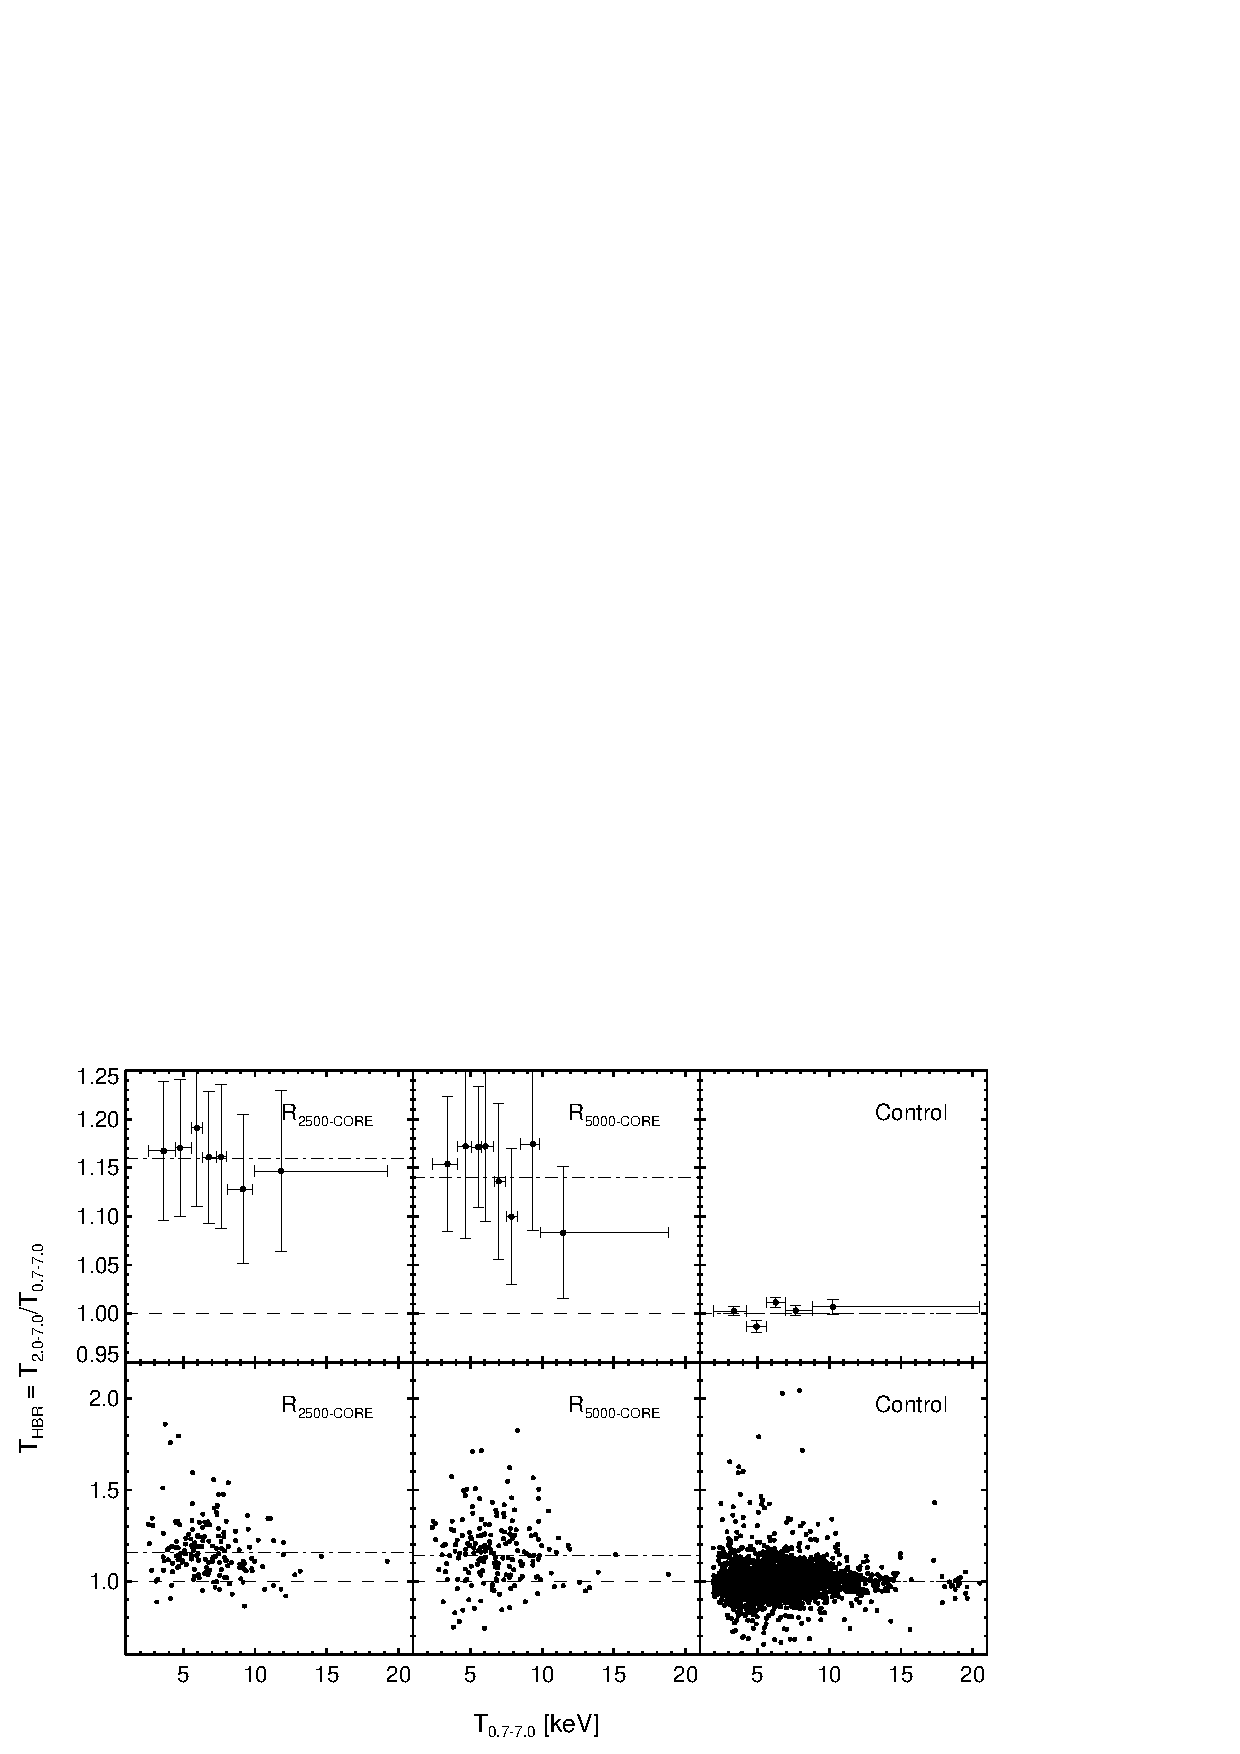
\includegraphics[scale=1.0]{ftxcount}
\caption{\small Best-fit temperatures for the hard bandpass,
\hard, divided by the full bandpass, \full plotted
against the full bandpass temperature. For binned data, each bin
contains 20 clusters, with the exception of the highest temperature
bin for R$_{5000-\text{CORE}}$ which contains 14 clusters; the
Simulated data bins contain 200 clusters with the last bin having 120
clusters. The line of equality is shown as a dashed line and the weighted
mean for the full sample is shown as a dashed-dotted line. Error
bars are omitted in the unbinned data for clarity.}
\label{fig:ftx}
\end{center}
\end{figure}

\clearpage
\begin{figure}[htp]
\begin{center}
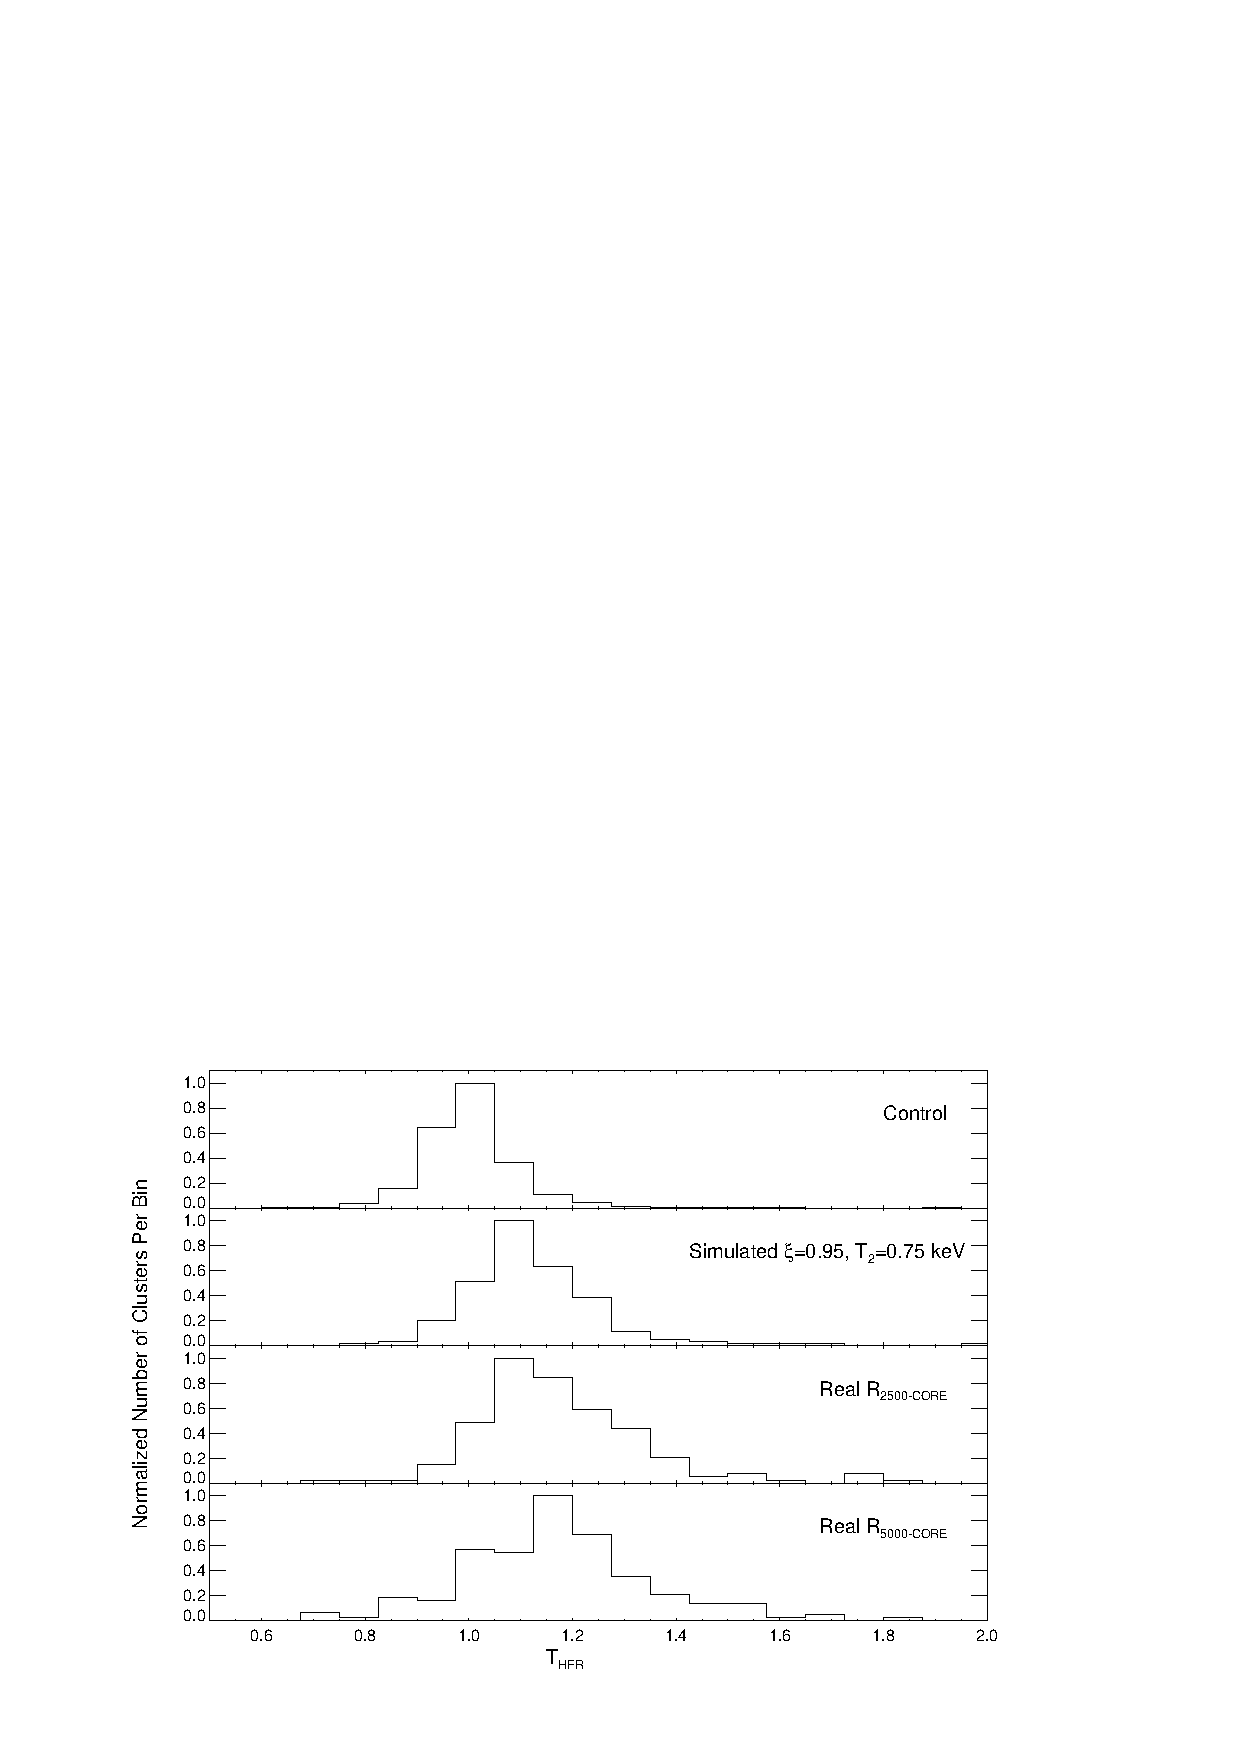
\includegraphics[scale=1.0]{ft_histo}
\caption{\small Normalized distributions for the simulated, control, 
R$_{2500-\text{CORE}}$, and R$_{5000-\text{CORE}}$ samples as a function of
\tf. The Simulated distribution  has been culled to only include
spectra for $\eta = 0.9$ and T$_{2}$ = 0.75 keV (see
\S\ref{sec:simulated} for discussion). Bins are 0.05 in width with a vertical line
drawn for the weighted-mean of \tf = 1.13 taken from the R$_{2500-\text{CORE}}$
sample. The simulated and real distributions are nearly log-normal
while the control distribution is roughly Gaussian.}
\label{fig:ft_histo}
\end{center}
\end{figure}

\clearpage
\begin{figure}[htp]
\begin{center}
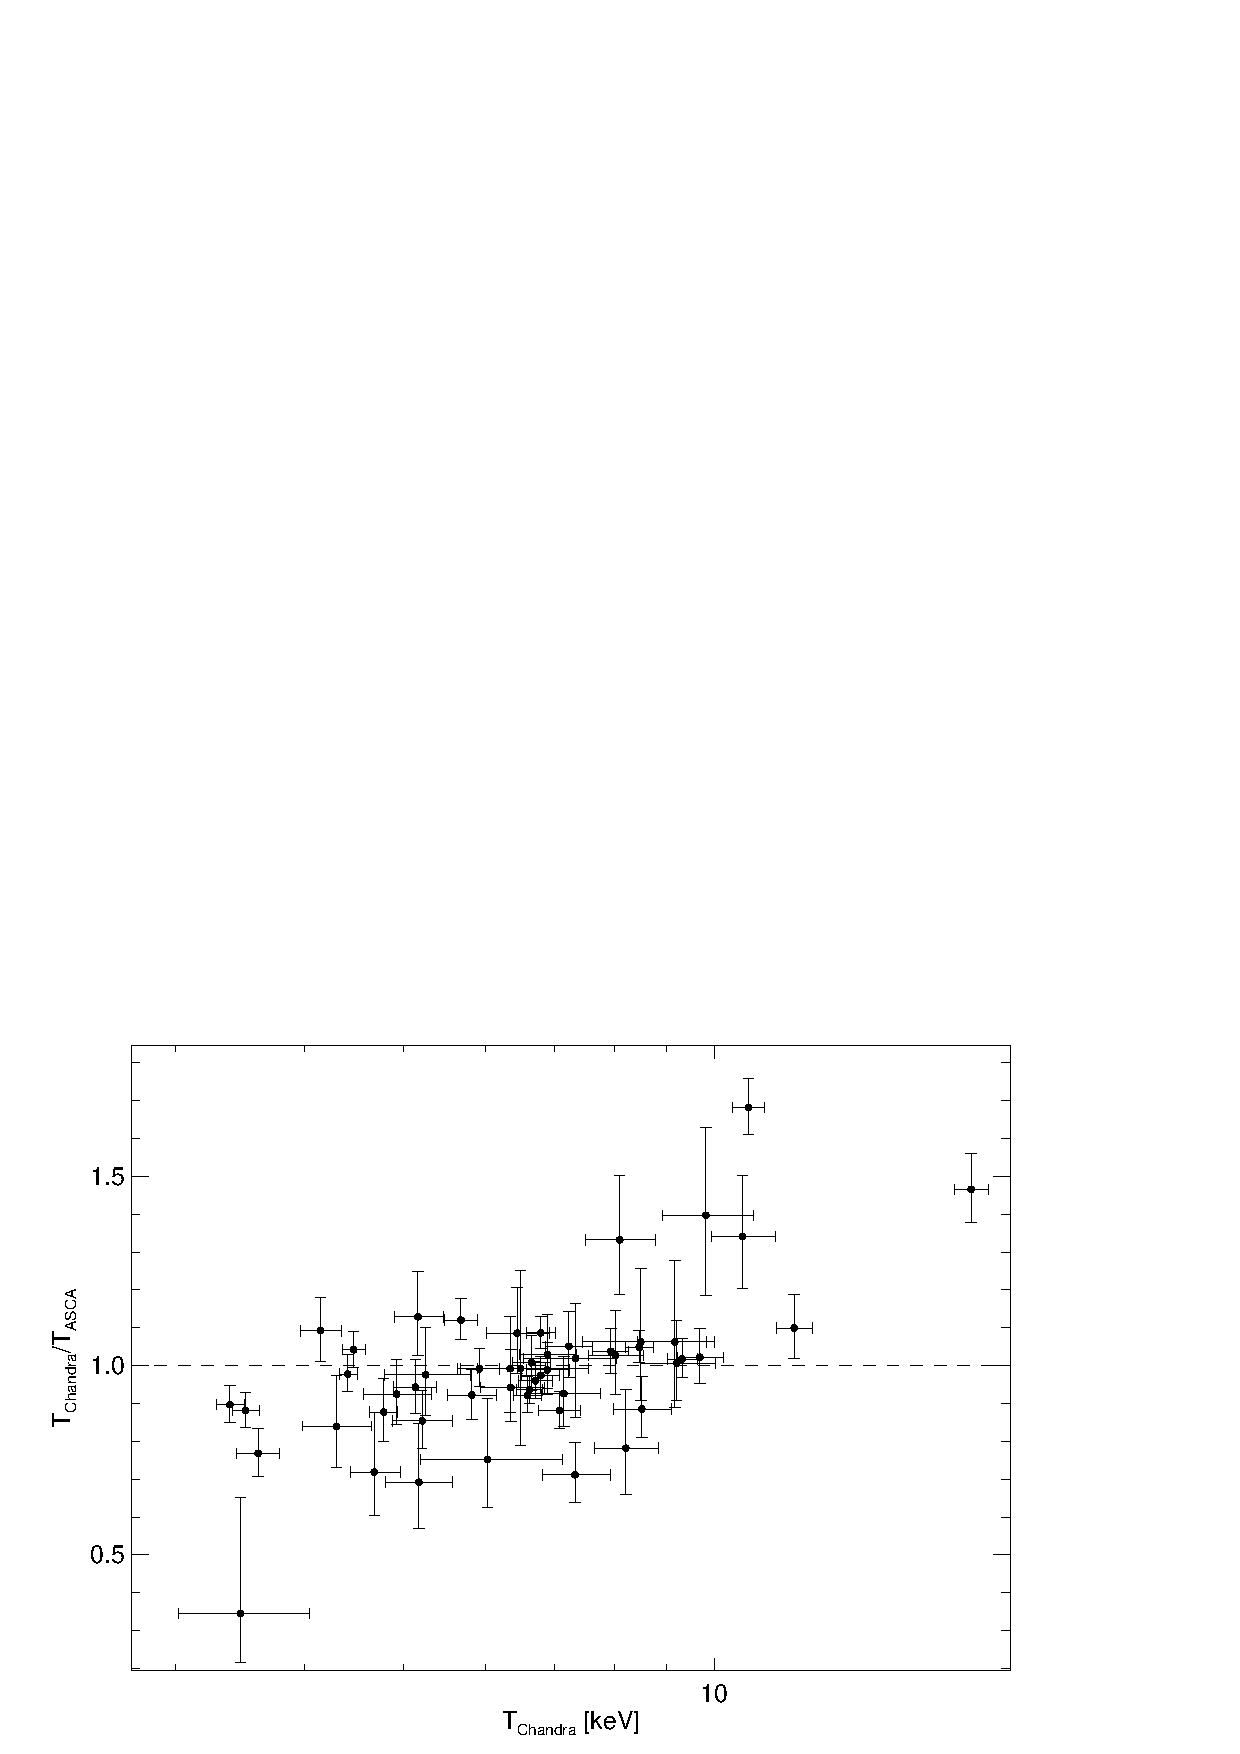
\includegraphics[scale=1.0]{asch}
\caption{\small Ratio of {\textit{ASCA}} temperatures taken from Don
Horner's thesis to {\textit{Chandra}} temperatures derived in this
work. We note a trend of hotter {\textit{ASCA}} temperatures for
clusters $> 10$ keV. The spurious point below 0.5 is MS
2053.7-0449 which has a poorly constrained {\textit{ASCA}}
temperature. Our derived temperature of $\sim$ 3.5 keV is in agreement
with recent work of \cite{2007astro.ph..3156M}.}
\label{fig:asch}
\end{center}
\end{figure}

\clearpage
\begin{figure}[htp]
\begin{center}
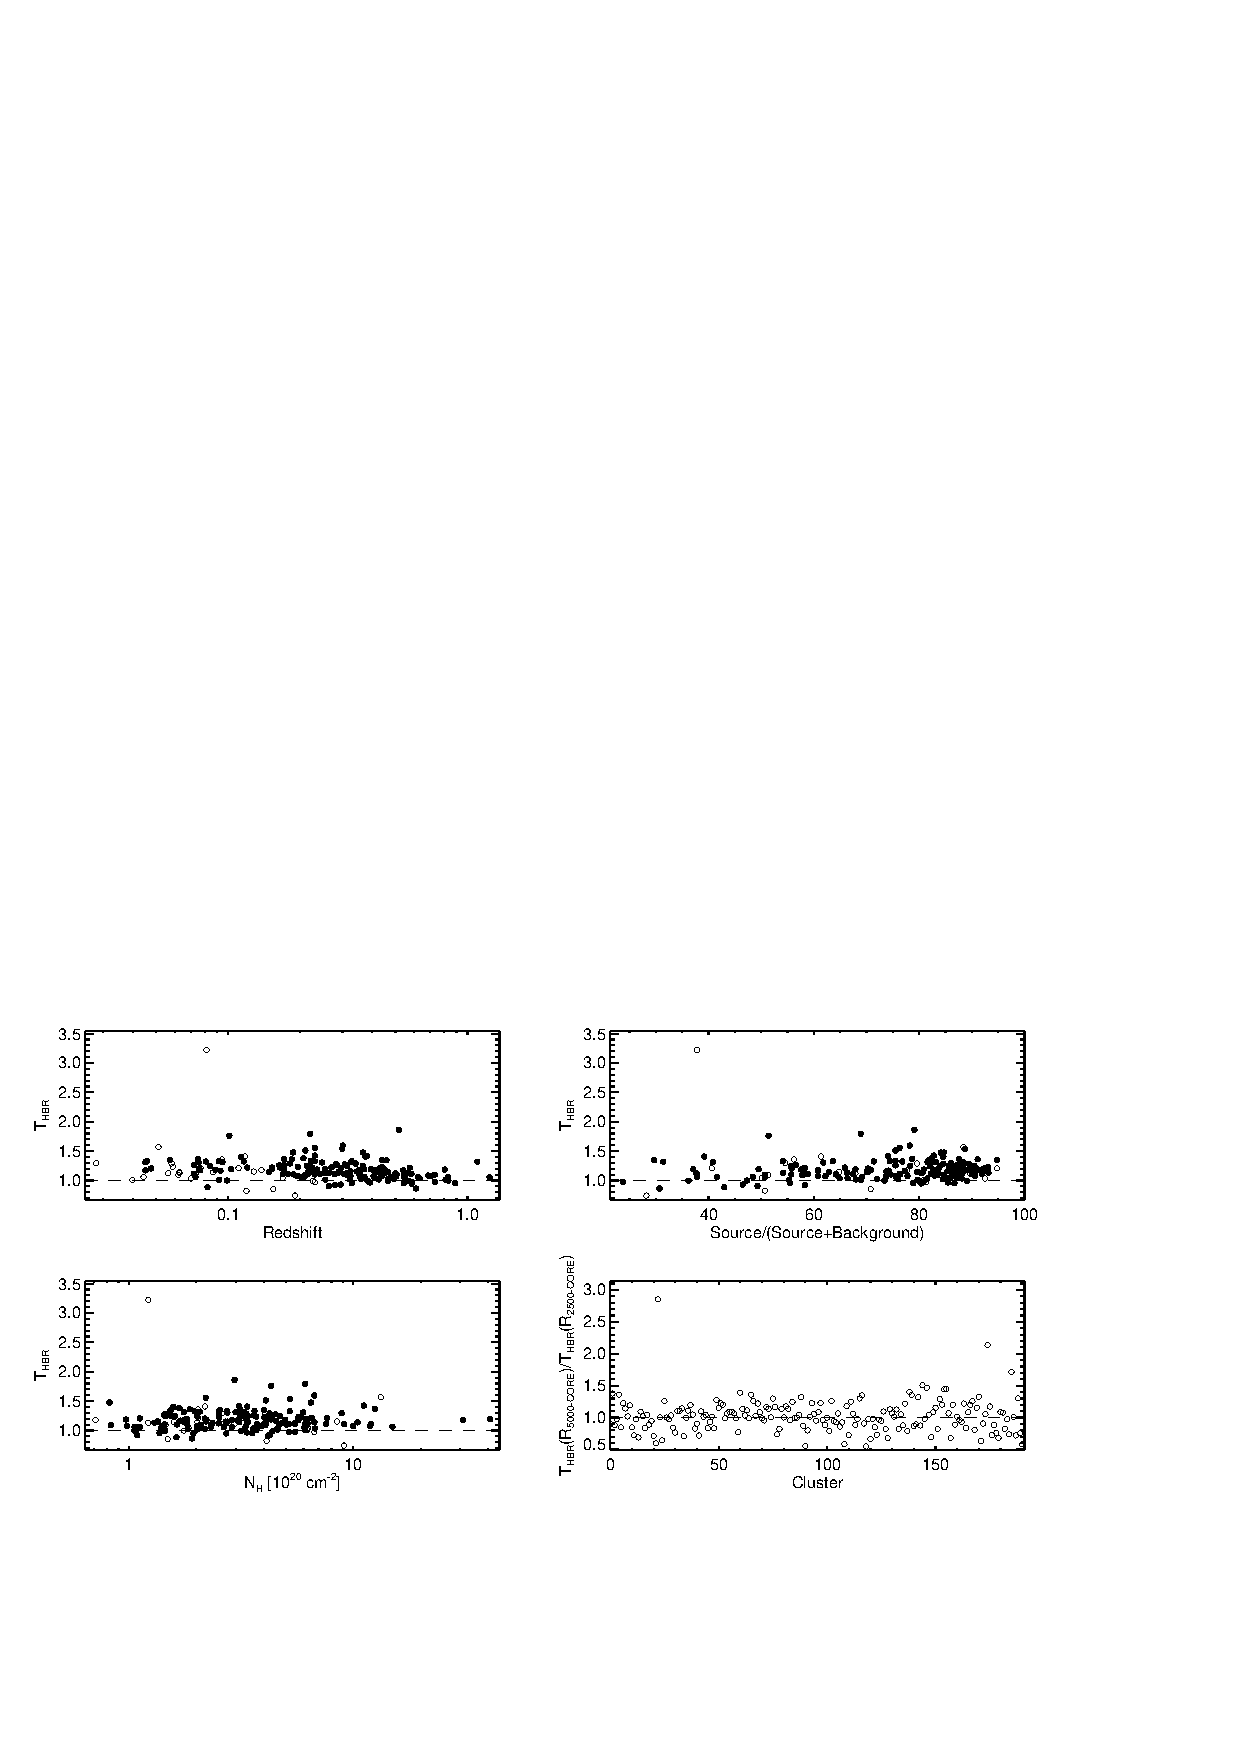
\includegraphics[scale=1.0]{sys}
\caption{\small Three possible sources of systematics are
plotted versus \tf plus a comparison of \tf for our two
physically motivated apertures, R$_{2500}$ and R$_{5000}$. Error bars
have been omitted in the last plot for clarity as they all cross the
line of equality. The trend in \tf with redshift is expected as the
2.0/(1+z) keV hard band lower boundary nears convergence with the 0.7
full band lower boundary which occurs at z $\sim 1.85$. We find no
other trends in the plotted relations.}
\label{fig:sys}
\end{center}
\end{figure}

\clearpage
\begin{figure}[htp]
\begin{center}
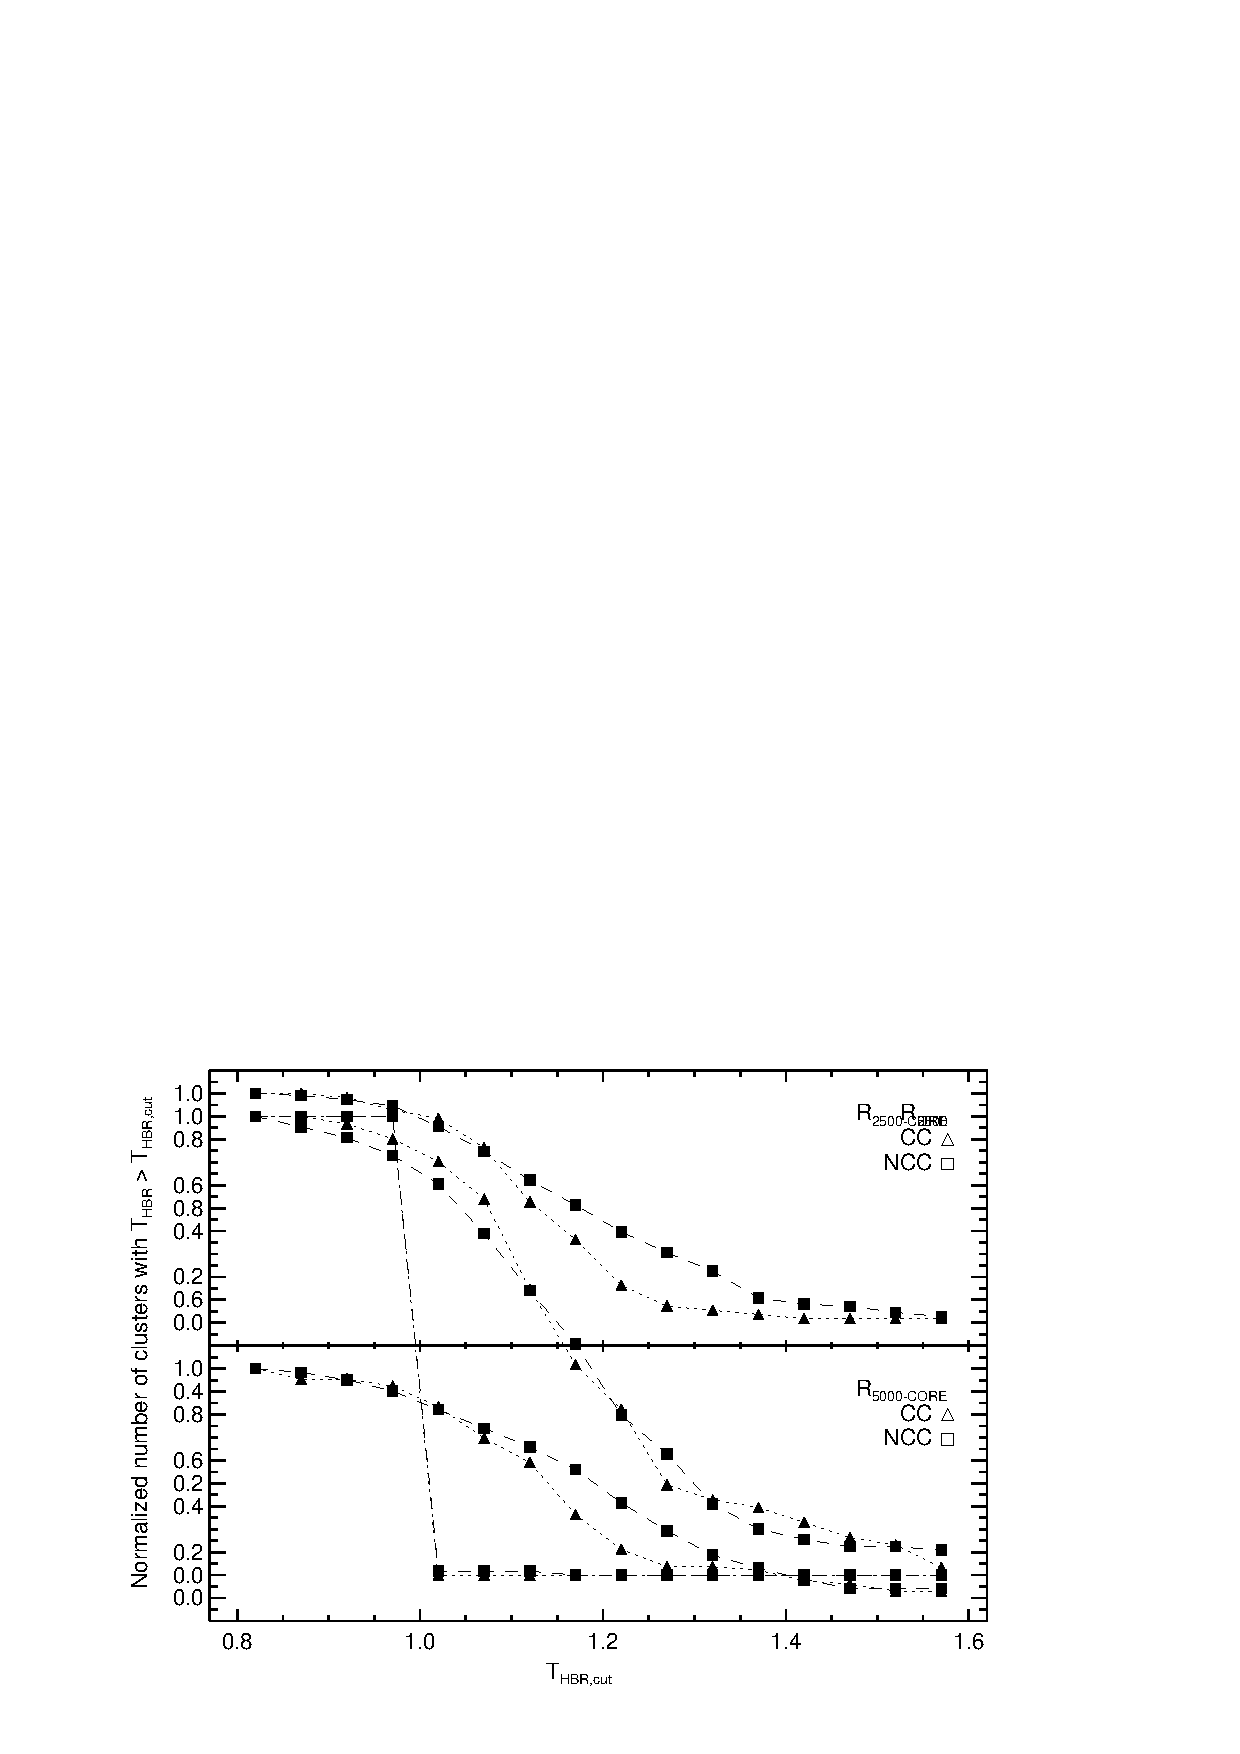
\includegraphics[scale=1.0]{cc_ncc_bin}
\caption{\small We have defined a cluster as having a cool core (CC)
when the temperature for the 50 kpc around the cluster center divided
by the temperature for R$_{5000-\text{CORE}}$ was less than 1 at the
$2\sigma$ level. We then take cuts in \tf at the $1\sigma$
level and ask how many CC and NCC clusters are above these cuts. The
number of CC clusters falls off more rapidly than NCC clusters in this
classification suggesting higher values of \tf prefer less
relaxed systems which do not have cool cores. This result is
insensitive to our choice of significance level in both the CC
classification and \tf cuts.}
\label{fig:cc_ncc_bin}
\end{center}
\end{figure}

%%%%%%%%%%
% Tables %
%%%%%%%%%%

\clearpage
\LongTables
\begin{deluxetable}{lcrrcccccccc}
\tablewidth{0pt}
\tabletypesize{\scriptsize}
\tablecaption{Summary of Sample\label{tab:sample}}
\tablehead{\colhead{Cluster} & \colhead{Obs.ID} & \colhead{R.A.} & \colhead{Dec.} & \colhead{ExpT} & \colhead{Mode} & \colhead{ACIS} & \colhead{z} & \colhead{L$_{bol.}$}\\
\colhead{ } & \colhead{ } & \colhead{hr:min:sec} & \colhead{$\degr:\arcmin:\arcsec$} & \colhead{ksec} & \colhead{ } & \colhead{ } & \colhead{ } & \colhead{$10^{45}$ $h_{70}^{-2}$ ergs s$^{-1}$}\\
\colhead{{(1)}} & \colhead{{(2)}} & \colhead{{(3)}} & \colhead{{(4)}} & \colhead{{(5)}} & \colhead{{(6)}} & \colhead{{(7)}} & \colhead{{(8)}} & \colhead{{(9)}}
}
\startdata
1E0657 56 & 3184 & 06:58:29.510 & -55:56:39.79 & 87.5 & VF & I3 & 0.2960 & 54.10\\
1E0657 56 & 5356 & 06:58:29.619 & -55:56:39.35 & 97.2 & VF & I2 & 0.2960 & 54.10\\
1E0657 56 & 5361 & 06:58:29.436 & -55:56:40.30 & 82.6 & VF & I3 & 0.2960 & 54.10\\
1RXS J2129.4-0741 & 3199 & 21:29:26.274 & -07:41:29.18 & 19.9 & VF & I3 & 0.5700 & 23.30\\
1RXS J2129.4-0741 & 3595 & 21:29:26.016 & -07:41:29.36 & 19.9 & VF & I3 & 0.5700 & 23.30\\
3C 220.1 &  839 & 09:32:40.218 & +79:06:29.46 & 18.9 &  F & S3 & 0.6100 &  9.67\\
3C 28.0 & 3233 & 00:55:50.401 & +26:24:36.47 & 49.7 & VF & I3 & 0.1952 &  5.42\\
3C 295 & 2254 & 14:11:20.280 & +52:12:10.55 & 90.9 & VF & I3 & 0.4641 & 10.70\\
3C 388 & 5295 & 18:44:02.365 & +45:33:29.31 & 30.7 & VF & I3 & 0.0917 &  0.72\\
4C 55.16 & 4940 & 08:34:54.923 & +55:34:21.15 & 96.0 & VF & S3 & 0.2420 &  8.01\\
ABELL 0068 & 3250 & 00:37:06.309 & +09:09:32.28 & 10.0 & VF & I3 & 0.2546 & 12.79\\
ABELL 0085 &  904 & 00:41:50.406 & -09:18:10.79 & 38.4 &  F & I0 & 0.0558 &  6.44\\
ABELL 0133 & 2203 & 01:02:41.756 & -21:52:49.79 & 35.5 &  F & S3 & 0.0558 &  1.29\\
ABELL 0267 & 1448 & 01:52:42.302 & +01:00:44.34 & 7.9 &  F & I3 & 0.2300 &  9.10\\
ABELL 0267 & 3580 & 01:52:42.170 & +01:00:45.63 & 19.9 & VF & I3 & 0.2300 &  9.10\\
ABELL 0370 &  515 & 02:39:53.169 & -01:34:36.96 & 88.0 &  F & S3 & 0.3747 & 12.45\\
ABELL 0383 & 2321 & 02:48:03.364 & -03:31:44.69 & 19.5 &  F & S3 & 0.1871 &  7.22\\
ABELL 0399 & 3230 & 02:57:54.931 & +13:01:58.41 & 48.6 & VF & I0 & 0.0716 &  3.97\\
ABELL 0478 & 1669 & 04:13:25.345 & +10:27:55.64 & 42.4 &  F & S3 & 0.0883 & 19.22\\
ABELL 0478 & 6102 & 04:13:25.214 & +10:27:55.13 & 10.0 & VF & I3 & 0.0883 & 19.22\\
ABELL 0496 & 3361 & 04:33:37.802 & -13:15:40.14 & 10.0 & VF & S3 & 0.0328 &  1.17\\
ABELL 0520 & 4215 & 04:54:09.711 & +02:55:23.69 & 66.3 & VF & I3 & 0.2020 & 12.20\\
ABELL 0521 &  430 & 04:54:07.004 & -10:13:26.72 & 39.1 & VF & S3 & 0.2533 &  9.39\\
ABELL 0576 & 3289 & 07:21:30.394 & +55:45:41.95 & 38.6 & VF & S3 & 0.0385 &  0.55\\
ABELL 0586 &  530 & 07:32:20.339 & +31:37:58.59 & 10.0 & VF & I3 & 0.1710 &  9.35\\
ABELL 0611 & 3194 & 08:00:56.832 & +36:03:24.09 & 36.1 & VF & S3 & 0.2880 & 12.50\\
ABELL 0644 $\dagger$ & 2211 & 08:17:25.225 & -07:30:40.03 & 29.7 & VF & I3 & 0.0698 &  8.07\\
ABELL 0665 & 3586 & 08:30:59.231 & +65:50:37.78 & 29.7 & VF & I3 & 0.1810 & 13.46\\
ABELL 0697 & 4217 & 08:42:57.549 & +36:21:57.65 & 19.5 & VF & I3 & 0.2820 & 26.49\\
ABELL 0773 & 5006 & 09:17:52.566 & +51:43:38.18 & 19.8 & VF & I3 & 0.2170 & 12.88\\
ABELL 0781 &  534 & 09:20:25.431 & +30:30:07.56 & 9.9 & VF & I3 & 0.2984 &  7.71\\
ABELL 0907 & 3185 & 09:58:21.880 & -11:03:52.20 & 48.0 & VF & I3 & 0.1527 &  7.37\\
ABELL 0963 &  903 & 10:17:03.744 & +39:02:49.17 & 36.3 &  F & S3 & 0.2056 & 12.24\\
ABELL 1060 & 2220 & 10:36:42.828 & -27:31:42.06 & 31.9 & VF & I3 & 0.0125 &  0.09\\
ABELL 1063S & 4966 & 22:48:44.294 & -44:31:48.37 & 26.7 & VF & I3 & 0.3540 & 79.90\\
ABELL 1068 & 1652 & 10:40:44.520 & +39:57:10.28 & 26.8 &  F & S3 & 0.1375 &  6.93\\
ABELL 1201 $\dagger$ & 4216 & 11:12:54.489 & +13:26:08.76 & 39.7 & VF & S3 & 0.1688 &  4.51\\
ABELL 1204 & 2205 & 11:13:20.419 & +17:35:38.45 & 23.6 & VF & I3 & 0.1706 &  6.91\\
ABELL 1361 $\dagger$ & 2200 & 11:43:39.827 & +46:21:21.40 & 16.7 &  F & S3 & 0.1171 &  3.13\\
ABELL 1413 & 5003 & 11:55:17.893 & +23:24:21.84 & 75.1 & VF & I2 & 0.1426 & 11.28\\
ABELL 1423 &  538 & 11:57:17.026 & +33:36:37.44 & 9.8 & VF & I3 & 0.2130 &  7.40\\
ABELL 1650 & 4178 & 12:58:41.499 & -01:45:44.32 & 27.3 & VF & S3 & 0.0843 &  5.25\\
ABELL 1651 & 4185 & 12:59:22.830 & -04:11:45.86 & 9.6 & VF & I3 & 0.0840 &  7.18\\
ABELL 1664 & 1648 & 13:03:42.478 & -24:14:44.55 & 9.8 & VF & S3 & 0.1276 &  4.01\\
ABELL 1682 & 3244 & 13:06:50.764 & +46:33:19.86 & 9.8 & VF & I3 & 0.2260 &  7.23\\
ABELL 1689 & 5004 & 13:11:29.474 & -01:20:25.17 & 19.9 & VF & I3 & 0.1843 & 31.82\\
ABELL 1758 & 2213 & 13:32:42.978 & +50:32:44.83 & 58.3 & VF & S3 & 0.2792 & 19.63\\
ABELL 1763 & 3591 & 13:35:17.957 & +40:59:55.80 & 19.6 & VF & I3 & 0.1866 &  9.21\\
ABELL 1795 $\dagger$ & 5289 & 13:48:52.645 & +26:35:25.00 & 15.0 & VF & I3 & 0.0625 &  9.61\\
ABELL 1835 &  495 & 14:01:01.951 & +02:52:43.18 & 19.5 &  F & S3 & 0.2532 & 48.70\\
ABELL 1914 & 3593 & 14:26:01.399 & +37:49:27.83 & 18.9 & VF & I3 & 0.1712 & 28.42\\
ABELL 1942 & 3290 & 14:38:21.878 & +03:40:12.97 & 57.6 & VF & I2 & 0.2240 &  2.25\\
ABELL 1991 & 3193 & 14:54:31.620 & +18:38:41.48 & 38.3 & VF & S3 & 0.0565 &  0.77\\
ABELL 2029 & 4977 & 15:10:56.139 & +05:44:40.96 & 77.9 &  F & S3 & 0.0765 & 18.15\\
ABELL 2029 & 6101 & 15:10:56.064 & +05:44:40.40 & 9.9 & VF & I3 & 0.0765 & 18.15\\
ABELL 2034 & 2204 & 15:10:11.003 & +33:30:46.46 & 53.9 & VF & I3 & 0.1130 &  6.29\\
ABELL 2069 & 4965 & 15:24:09.181 & +29:53:18.05 & 55.4 & VF & I2 & 0.1160 &  3.94\\
ABELL 2104 &  895 & 15:40:08.591 & -03:18:07.14 & 49.2 &  F & S3 & 0.1554 &  7.40\\
ABELL 2111 &  544 & 15:39:41.432 & +34:25:12.26 & 10.3 &  F & I3 & 0.2300 &  5.31\\
ABELL 2124 & 3238 & 15:44:59.131 & +36:06:34.11 & 19.4 & VF & S3 & 0.0658 &  0.52\\
ABELL 2125 & 2207 & 15:41:14.154 & +66:15:57.20 & 81.5 & VF & I3 & 0.2465 &  0.83\\
ABELL 2147 & 3211 & 16:02:13.476 & +15:57:58.32 & 17.9 & VF & I1 & 0.0356 &  0.72\\
ABELL 2163 & 1653 & 16:15:45.705 & -06:09:00.62 & 71.1 & VF & I1 & 0.1695 & 47.39\\
ABELL 2199 &  497 & 16:28:38.249 & +39:33:04.28 & 19.5 &  F & S3 & 0.0300 &  1.52\\
ABELL 2204 $\dagger$ &  499 & 16:32:46.986 & +05:34:30.89 & 10.1 &  F & S3 & 0.1524 & 29.00\\
ABELL 2204 $\dagger$ & 6104 & 16:32:46.944 & +05:34:31.22 & 9.6 & VF & I3 & 0.1524 & 29.00\\
ABELL 2218 & 1666 & 16:35:50.831 & +66:12:42.31 & 48.6 & VF & I0 & 0.1713 &  8.47\\
ABELL 2219 &  896 & 16:40:21.069 & +46:42:29.07 & 42.3 &  F & S3 & 0.2256 & 39.69\\
ABELL 2244 & 4179 & 17:02:42.579 & +34:03:37.34 & 57.0 & VF & S3 & 0.0967 &  6.43\\
ABELL 2255 &  894 & 17:12:40.385 & +64:03:50.63 & 39.4 &  F & I3 & 0.0805 &  6.08\\
ABELL 2259 & 3245 & 17:20:08.299 & +27:40:11.53 & 10.0 & VF & I3 & 0.1640 &  5.64\\
ABELL 2261 & 5007 & 17:22:27.254 & +32:07:58.60 & 24.3 & VF & I3 & 0.2240 & 19.71\\
ABELL 2294 & 3246 & 17:24:10.149 & +85:53:09.77 & 10.0 & VF & I3 & 0.1780 & 10.31\\
ABELL 2319 $\dagger$ & 3231 & 19:21:12.280 & +43:55:57.89 & 14.4 & VF & I1 & 0.0562 & 12.23\\
ABELL 2384 & 4202 & 21:52:21.178 & -19:32:51.90 & 31.5 & VF & I3 & 0.0945 &  2.14\\
ABELL 2390 & 4193 & 21:53:36.825 & +17:41:44.38 & 95.1 & VF & S3 & 0.2301 & 37.84\\
ABELL 2409 & 3247 & 22:00:52.567 & +20:58:34.11 & 10.2 & VF & I3 & 0.1479 &  7.35\\
ABELL 2537 & 4962 & 23:08:22.313 & -02:11:29.88 & 36.2 & VF & S3 & 0.2950 & 11.31\\
ABELL 2550 & 2225 & 23:11:35.806 & -21:44:46.70 & 59.0 & VF & S3 & 0.1543 &  0.83\\
ABELL 2554 $\dagger$ & 1696 & 23:12:19.939 & -21:30:09.84 & 19.9 & VF & S3 & 0.1103 &  1.65\\
ABELL 2556 $\dagger$ & 2226 & 23:13:01.413 & -21:38:04.47 & 19.9 & VF & S3 & 0.0862 &  2.10\\
ABELL 2589 & 3210 & 23:23:57.315 & +16:46:38.43 & 13.7 & VF & S3 & 0.0415 &  0.90\\
ABELL 2597 &  922 & 23:25:19.779 & -12:07:27.63 & 39.4 &  F & S3 & 0.0854 &  3.36\\
ABELL 2626 & 3192 & 23:36:30.452 & +21:08:47.36 & 24.8 & VF & S3 & 0.0573 &  0.91\\
ABELL 2634 & 4816 & 23:38:29.397 & +27:01:53.14 & 49.5 & VF & S3 & 0.0314 &  0.06\\
ABELL 2667 & 2214 & 23:51:39.395 & -26:05:02.75 & 9.6 & VF & S3 & 0.2300 & 22.93\\
ABELL 2670 & 4959 & 23:54:13.687 & -10:25:08.85 & 39.6 & VF & I3 & 0.0763 &  1.45\\
ABELL 2744 & 2212 & 00:14:14.396 & -30:22:40.04 & 24.8 & VF & S3 & 0.3080 & 27.95\\
ABELL 3112 & 2516 & 03:17:57.681 & -44:14:17.16 & 16.9 & VF & S3 & 0.0720 &  4.68\\
ABELL 3158 & 3201 & 03:42:54.675 & -53:37:24.36 & 24.8 & VF & I3 & 0.0580 &  3.46\\
ABELL 3266 &  899 & 04:31:14.960 & -61:27:32.23 & 29.8 & VF & I1 & 0.0590 &  3.46\\
ABELL 3558 & 1646 & 13:27:56.854 & -31:29:43.78 & 14.4 & VF & S3 & 0.0480 &  1.96\\
ABELL 3562 $\dagger$ & 4167 & 13:33:36.566 & -31:40:27.78 & 19.3 & VF & I2 & 0.0490 &  1.18\\
ABELL 3571 & 4203 & 13:47:28.434 & -32:51:52.45 & 34.0 & VF & S3 & 0.0391 &  1.86\\
ABELL 3667 & 5751 & 20:12:41.231 & -56:50:35.70 & 128.9 & VF & I3 & 0.0556 &  4.43\\
ABELL 4038 & 4992 & 23:47:44.668 & -28:08:19.07 & 33.5 & VF & I2 & 0.0300 &  1.03\\
AC 114 & 1562 & 22:58:48.196 & -34:47:56.89 & 72.5 &  F & S3 & 0.3120 & 11.51\\
CL 0024+17 &  929 & 00:26:35.996 & +17:09:45.37 & 39.8 &  F & S3 & 0.3940 &  3.12\\
CL 1221+4918 & 1662 & 12:21:26.709 & +49:18:21.60 & 79.1 & VF & I3 & 0.7000 &  8.04\\
CL J0030+2618 & 5762 & 00:30:33.571 & +26:18:09.45 & 17.9 & VF & I3 & 0.5000 &  3.66\\
CL J0152-1357 &  913 & 01:52:42.141 & -13:57:59.71 & 36.5 &  F & I3 & 0.8310 & 13.58\\
CL J0542.8-4100 &  914 & 05:42:49.994 & -40:59:58.50 & 50.4 &  F & I3 & 0.6300 &  6.73\\
CL J0848+4456 & 1708 & 08:48:48.235 & +44:56:17.30 & 61.4 & VF & I1 & 0.5740 &  0.73\\
CL J0848+4456 &  927 & 08:48:47.233 & +44:56:17.13 & 125.1 & VF & I1 & 0.5740 &  0.73\\
CL J1113.1-2615 &  915 & 11:13:05.167 & -26:15:40.43 & 104.6 &  F & I3 & 0.7300 &  2.64\\
CL J1213+0253 & 4934 & 12:13:34.948 & +02:53:45.45 & 18.9 & VF & I3 & 0.4090 &  1.48\\
CL J1226.9+3332 & 3180 & 12:26:58.058 & +33:32:46.87 & 31.7 & VF & I3 & 0.8900 & 32.65\\
CL J1226.9+3332 & 5014 & 12:26:58.372 & +33:32:47.67 & 32.7 & VF & I3 & 0.8900 & 32.65\\
CL J1641+4001 & 3575 & 16:41:53.704 & +40:01:44.40 & 46.5 & VF & I3 & 0.4640 &  1.45\\
CL J2302.8+0844 &  918 & 23:02:48.156 & +08:43:52.74 & 108.6 &  F & I3 & 0.7300 &  2.71\\
CYGNUS A &  360 & 19:59:28.381 & +40:44:01.98 & 34.7 &  F & S3 & 0.0561 &  4.03\\
ESO 3060170 & 3189 & 05:40:06.679 & -40:50:11.97 & 14.1 & VF & I0 & 0.0358 &  0.32\\
ESO 5520200 & 3206 & 04:54:52.318 & -18:06:56.52 & 23.9 & VF & I3 & 0.0314 &  0.11\\
EXO 0422-086 $\dagger$ & 4183 & 04:25:51.271 & -08:33:36.42 & 10.0 & VF & I3 & 0.0397 &  1.02\\
HERCULES A $\dagger$ & 1625 & 16:51:08.161 & +04:59:32.44 & 14.8 & VF & S3 & 0.1541 &  3.75\\
HYDRA A & 4970 & 09:18:05.985 & -12:05:43.94 & 98.8 & VF & S3 & 0.0549 &  3.92\\
IRAS 09104+4109 &  509 & 09:13:45.481 & +40:56:27.49 & 9.1 &  F & S3 & 0.4420 & 25.41\\
LYNX E & 17081 & 08:48:58.841 & +44:51:51.63 & 61.4 & VF & I2 & 0.5740 &  0.47\\
LYNX E & 9271 & 08:48:58.858 & +44:51:51.46 & 125.1 & VF & I2 & 1.2600 &  0.47\\
MACS J0011.7-1523 & 6105 & 00:11:42.957 & -15:23:20.46 & 37.3 & VF & I3 & 0.3600 & 13.01\\
MACS J0025.4-1222 & 3251 & 00:25:29.368 & -12:22:38.05 & 19.3 & VF & I3 & 0.5843 & 13.77\\
MACS J0025.4-1222 & 5010 & 00:25:29.332 & -12:22:37.61 & 24.8 & VF & I3 & 0.5843 & 13.77\\
MACS J0159.8-0849 & 3265 & 01:59:49.320 & -08:50:00.41 & 17.9 & VF & I3 & 0.4050 & 31.67\\
MACS J0159.8-0849 & 6106 & 01:59:49.422 & -08:50:00.42 & 35.3 & VF & I3 & 0.4050 & 31.67\\
MACS J0242.5-2132 & 3266 & 02:42:35.906 & -21:32:26.30 & 11.9 & VF & I3 & 0.3140 & 20.18\\
MACS J0257.1-2325 & 1654 & 02:57:09.130 & -23:26:05.85 & 19.8 &  F & I3 & 0.5053 & 24.60\\
MACS J0257.1-2325 & 3581 & 02:57:09.188 & -23:26:06.70 & 18.5 & VF & I3 & 0.5053 & 24.60\\
MACS J0257.6-2209 & 3267 & 02:57:41.024 & -22:09:11.12 & 20.5 & VF & I3 & 0.3224 & 12.29\\
MACS J0329.6-0211 & 3257 & 03:29:41.616 & -02:11:49.15 & 9.9 & VF & I3 & 0.4500 & 17.70\\
MACS J0329.6-0211 & 3582 & 03:29:41.622 & -02:11:46.82 & 19.9 & VF & I3 & 0.4500 & 17.70\\
MACS J0329.6-0211 & 6108 & 03:29:41.681 & -02:11:47.57 & 39.6 & VF & I3 & 0.4500 & 17.70\\
MACS J0404.6+1109 & 3269 & 04:04:32.491 & +11:08:02.10 & 21.8 & VF & I3 & 0.3548 &  4.08\\
MACS J0417.5-1154 & 3270 & 04:17:34.686 & -11:54:32.71 & 12.0 & VF & I3 & 0.4400 & 43.38\\
MACS J0429.6-0253 & 3271 & 04:29:36.088 & -02:53:09.02 & 23.2 & VF & I3 & 0.3990 & 16.57\\
MACS J0451.9+0006 & 5815 & 04:51:54.291 & +00:06:20.20 & 10.2 & VF & I3 & 0.4300 &  9.29\\
MACS J0547.0-3904 & 3273 & 05:47:01.582 & -39:04:28.24 & 21.7 & VF & I3 & 0.2100 &  2.64\\
MACS J0717.5+3745 & 1655 & 07:17:32.443 & +37:45:29.83 & 19.9 &  F & I3 & 0.5480 & 47.95\\
MACS J0717.5+3745 & 4200 & 07:17:31.651 & +37:45:18.95 & 59.2 & VF & I3 & 0.5480 & 47.95\\
MACS J0744.8+3927 & 3197 & 07:44:52.801 & +39:27:25.40 & 20.2 & VF & I3 & 0.6860 & 29.94\\
MACS J0744.8+3927 & 3585 & 07:44:52.779 & +39:27:24.90 & 19.9 & VF & I3 & 0.6860 & 29.94\\
MACS J0744.8+3927 & 6111 & 07:44:52.842 & +39:27:26.28 & 49.5 & VF & I3 & 0.6860 & 29.94\\
MACS J0911.2+1746 & 3587 & 09:11:11.291 & +17:46:31.75 & 17.9 & VF & I3 & 0.5409 & 12.16\\
MACS J0949+1708 & 3274 & 09:49:51.824 & +17:07:05.62 & 14.3 & VF & I3 & 0.3820 & 20.93\\
MACS J1115.8+0129 & 3275 & 11:15:52.048 & +01:29:56.56 & 15.9 & VF & I3 & 0.1200 &  2.48\\
MACS J1131.8-1955 & 3276 & 11:31:56.011 & -19:55:55.85 & 13.9 & VF & I3 & 0.3070 & 18.48\\
MACS J1149.5+2223 & 1656 & 11:49:35.466 & +22:23:53.06 & 18.5 & VF & I3 & 0.1761 &  2.76\\
MACS J1149.5+2223 & 3589 & 11:49:35.848 & +22:23:55.04 & 20.0 & VF & I3 & 0.1761 &  2.76\\
MACS J1206.2-0847 & 3277 & 12:06:12.276 & -08:48:02.40 & 23.5 & VF & I3 & 0.4400 & 40.49\\
MACS J1226.8+2153 & 3590 & 12:26:51.207 & +21:49:55.22 & 19.0 & VF & I3 & 0.3700 &  3.21\\
MACS J1311.0-0310 & 3258 & 13:11:01.665 & -03:10:39.50 & 14.9 & VF & I3 & 0.4940 & 13.08\\
MACS J1311.0-0310 & 6110 & 13:11:01.647 & -03:10:37.78 & 63.2 & VF & I3 & 0.4940 & 13.08\\
MACS J1319+7003 & 3278 & 13:20:08.370 & +70:04:33.81 & 21.6 & VF & I3 & 0.3275 &  8.00\\
MACS J1427.6-2521 & 3279 & 14:27:39.389 & -25:21:04.66 & 16.9 & VF & I3 & 0.2200 &  2.41\\
MACS J1621.3+3810 & 3254 & 16:21:24.759 & +38:10:07.18 & 9.8 & VF & I3 & 0.4650 & 14.64\\
MACS J1621.3+3810 & 3594 & 16:21:24.933 & +38:10:06.57 & 19.7 & VF & I3 & 0.4610 & 14.64\\
MACS J1621.3+3810 & 6109 & 16:21:24.742 & +38:10:08.92 & 37.5 & VF & I3 & 0.4610 & 14.64\\
MACS J1621.3+3810 & 6172 & 16:21:24.849 & +38:10:08.72 & 29.8 & VF & I3 & 0.4610 & 14.64\\
MACS J1824.3+4309 & 3255 & 18:24:18.444 & +43:09:43.39 & 14.9 & VF & I3 & 0.4870 &  2.81\\
MACS J1931.8-2634 & 3282 & 19:31:49.656 & -26:34:33.99 & 13.6 & VF & I3 & 0.3520 & 32.00\\
MACS J2211.7-0349 & 3284 & 22:11:45.856 & -03:49:37.24 & 17.7 & VF & I3 & 0.2700 & 25.67\\
MACS J2214.9-1359 & 3259 & 22:14:57.467 & -14:00:09.35 & 19.5 & VF & I3 & 0.5026 & 26.01\\
MACS J2214.9-1359 & 5011 & 22:14:57.515 & -14:00:10.68 & 18.5 & VF & I3 & 0.5026 & 26.01\\
MACS J2228+2036 & 3285 & 22:28:33.241 & +20:37:11.42 & 19.9 & VF & I3 & 0.4120 & 19.44\\
MACS J2229.7-2755 & 3286 & 22:29:45.358 & -27:55:38.41 & 16.4 & VF & I3 & 0.3240 & 14.89\\
MACS J2245.0+2637 & 3287 & 22:45:04.547 & +26:38:07.88 & 16.9 & VF & I3 & 0.3040 & 12.19\\
MACS J2311+0338 & 3288 & 23:11:33.213 & +03:38:06.51 & 13.6 & VF & I3 & 0.2998 & 12.09\\
MKW 04 & 3234 & 12:04:27.218 & +01:53:42.79 & 30.0 & VF & S3 & 0.0198 &  0.08\\
MS 0016.9+1609 &  520 & 00:18:33.503 & +16:26:12.99 & 67.4 & VF & I3 & 0.5410 & 32.79\\
MS 0302.7+1658 &  525 & 03:05:31.614 & +17:10:02.06 & 10.0 & VF & I3 & 0.4240 &  3.22\\
MS 0440.5+0204 $\dagger$ & 4196 & 04:43:09.952 & +02:10:18.70 & 59.4 & VF & S3 & 0.1900 &  2.95\\
MS 0451.6-0305 &  902 & 04:54:11.004 & -03:00:52.19 & 44.2 &  F & S3 & 0.5386 & 36.16\\
MS 0735.6+7421 & 4197 & 07:41:44.245 & +74:14:38.23 & 45.5 & VF & S3 & 0.2160 &  8.97\\
MS 0839.8+2938 & 2224 & 08:42:55.969 & +29:27:26.97 & 29.8 &  F & S3 & 0.1940 &  4.14\\
MS 0906.5+1110 &  924 & 09:09:12.753 & +10:58:32.00 & 29.7 & VF & I3 & 0.1630 &  4.88\\
MS 1006.0+1202 &  925 & 10:08:47.194 & +11:47:55.99 & 29.4 & VF & I3 & 0.2210 &  7.56\\
MS 1008.1-1224 &  926 & 10:10:32.312 & -12:39:56.80 & 44.2 & VF & I3 & 0.3010 & 12.68\\
MS 1054.5-0321 &  512 & 10:56:58.499 & -03:37:32.76 & 89.1 &  F & S3 & 0.8300 & 27.43\\
MS 1455.0+2232 & 4192 & 14:57:15.088 & +22:20:32.49 & 91.9 & VF & I3 & 0.2590 & 15.00\\
MS 1621.5+2640 &  546 & 16:23:35.522 & +26:34:25.67 & 30.1 &  F & I3 & 0.4260 &  6.95\\
MS 2053.7-0449 & 1667 & 20:56:21.295 & -04:37:46.61 & 44.5 & VF & I3 & 0.5830 &  2.82\\
MS 2053.7-0449 &  551 & 20:56:21.264 & -04:37:46.80 & 44.3 &  F & I3 & 0.5830 &  2.82\\
MS 2137.3-2353 & 4974 & 21:40:15.178 & -23:39:40.71 & 57.4 & VF & S3 & 0.3130 & 17.51\\
OPHIUCHUS & 3200 & 17:12:27.731 & -23:22:06.74 & 50.5 &  F & S3 & 0.0280 &  3.90\\
PKS 0745-191 &  508 & 07:47:31.140 & -19:17:38.98 & 28.0 &  F & S3 & 0.1028 & 24.83\\
PKS 0745-191 & 6103 & 07:47:31.295 & -19:17:40.50 & 10.3 & VF & I3 & 0.1028 & 24.83\\
RBS 0797 & 2202 & 09:47:12.971 & +76:23:13.90 & 11.7 & VF & I3 & 0.3540 & 37.93\\
RDCS 1252-29 & 4198 & 12:52:54.221 & -29:27:21.01 & 163.4 & VF & I3 & 1.2370 &  2.80\\
RX J0439+0520 &  527 & 04:39:02.218 & +05:20:43.11 & 9.6 & VF & I3 & 0.2080 &  5.45\\
RX J0439.0+0715 & 1449 & 04:39:00.710 & +07:16:08.15 & 6.3 &  F & I3 & 0.2300 & 10.98\\
RX J0439.0+0715 & 3583 & 04:39:00.710 & +07:16:07.82 & 19.2 & VF & I3 & 0.2300 & 10.98\\
RX J0647.7+7015 & 3196 & 06:47:50.029 & +70:14:50.15 & 19.3 & VF & I3 & 0.5840 & 27.91\\
RX J0647.7+7015 & 3584 & 06:47:49.919 & +70:14:54.91 & 20.0 & VF & I3 & 0.5840 & 27.91\\
RX J0819.6+6336 $\dagger$ & 2199 & 08:19:26.007 & +63:37:26.53 & 14.9 &  F & S3 & 0.1190 &  1.27\\
RX J0820.9+0752 & 1647 & 08:21:02.180 & +07:51:48.42 & 9.4 &  F & S3 & 0.1100 &  1.01\\
RX J0910+5422 & 2452 & 09:10:44.478 & +54:22:04.26 & 65.3 & VF & I3 & 1.1000 &  1.48\\
RX J1053+5735 & 4936 & 10:53:39.844 & +57:35:18.42 & 92.2 &  F & S3 & 1.1400 &  2.44\\
RX J1347.5-1145 & 3592 & 13:47:30.593 & -11:45:10.05 & 57.7 & VF & I3 & 0.4510 & 125.14\\
RX J1347.5-1145 &  507 & 13:47:30.632 & -11:45:09.78 & 10.0 &  F & S3 & 0.4510 & 125.14\\
RX J1350+6007 & 2229 & 13:50:48.038 & +60:07:08.39 & 58.3 & VF & I3 & 0.8040 &  2.38\\
RX J1423.8+2404 & 1657 & 14:23:47.759 & +24:04:40.95 & 18.5 & VF & I3 & 0.5450 & 23.77\\
RX J1423.8+2404 & 4195 & 14:23:47.942 & +24:04:43.09 & 115.6 & VF & S3 & 0.5450 & 23.77\\
RX J1504.1-0248 & 5793 & 15:04:07.415 & -02:48:15.70 & 39.2 & VF & I3 & 0.2150 & 51.25\\
RX J1525+0958 & 1664 & 15:24:39.729 & +09:57:44.42 & 50.9 & VF & I3 & 0.5160 &  3.41\\
RX J1532.9+3021 & 1649 & 15:32:53.781 & +30:20:58.72 & 9.4 & VF & S3 & 0.3450 & 28.34\\
RX J1532.9+3021 & 1665 & 15:32:53.817 & +30:20:58.34 & 10.0 & VF & I3 & 0.3450 & 28.34\\
RX J1716.9+6708 &  548 & 17:16:49.015 & +67:08:25.80 & 51.7 &  F & I3 & 0.8100 &  9.00\\
RX J1720.1+2638 & 4361 & 17:20:09.941 & +26:37:29.11 & 25.7 & VF & I3 & 0.1640 & 14.50\\
RX J1720.2+3536 & 3280 & 17:20:16.792 & +35:36:26.08 & 20.8 & VF & I3 & 0.3913 & 16.44\\
RX J1720.2+3536 & 6107 & 17:20:16.908 & +35:36:26.43 & 33.9 & VF & I3 & 0.3913 & 16.44\\
RX J1720.2+3536 & 7225 & 17:20:16.947 & +35:36:23.78 & 2.0 & VF & I3 & 0.3913 & 16.44\\
RX J2129.6+0005 &  552 & 21:29:39.944 & +00:05:18.83 & 10.0 & VF & I3 & 0.2350 & 14.82\\
SERSIC 159-03 & 1668 & 23:13:58.764 & -42:43:34.70 & 9.9 & VF & S3 & 0.0580 &  1.97\\
V 1121.0+2327 & 1660 & 11:20:57.195 & +23:26:27.60 & 71.3 & VF & I3 & 0.5600 &  3.13\\
ZWCL 1215 & 4184 & 12:17:40.787 & +03:39:39.42 & 12.1 & VF & I3 & 0.0750 &  3.71\\
ZWCL 1358+6245 &  516 & 13:59:50.526 & +62:31:04.57 & 54.1 &  F & S3 & 0.3280 & 13.45\\
ZWCL 1953 & 1659 & 08:50:06.677 & +36:04:16.16 & 24.9 &  F & I3 & 0.3800 & 18.30\\
ZWCL 3146 &  909 & 10:23:39.735 & +04:11:08.05 & 46.0 &  F & I3 & 0.2900 & 43.20\\
ZWCL 5247 &  539 & 12:34:21.928 & +09:47:02.83 & 9.3 & VF & I3 & 0.2290 &  4.57\\
ZWCL 7160 &  543 & 14:57:15.158 & +22:20:33.85 & 9.9 &  F & I3 & 0.2578 & 15.09\\
ZWICKY 2701 & 3195 & 09:52:49.183 & +51:53:05.27 & 26.9 & VF & S3 & 0.2100 &  6.61\\
ZwCL 1332.8+5043 & 5772 & 13:34:20.698 & +50:31:04.64 & 19.5 & VF & I3 & 0.6200 &  4.82\\
\enddata
\tablecomments{(1) Cluster name, (2) CDA observation identification number, (3) centroid R.A., (4) centroid Dec., (5) nominal exposure time, (6) observing mode, (7) CCD location of centroid, (8) redshift, (9) NRAO absorbing Galactic neutral hydrogen column density, (10) fiducial temperature, (11) fiducial abundance, (12) bolometric luminosity. $\dagger$ indicates clusters analyzed within r$_{5000}$ only.}
\end{deluxetable}

%%%%%%%%%%%%%%%%%%%%%%%%%%%%%%%%
% Comparison of Tfrac for wavg %
%%%%%%%%%%%%%%%%%%%%%%%%%%%%%%%%

\begin{deluxetable}{c|ccc|ccc}
\tabletypesize{\scriptsize}
\tablecaption{Weighted averages for various apertures\label{tab:wavg}}
\tablewidth{0pt}
\tablehead{
\colhead{Aperture} & 
\colhead{[0.7-7.0]} & \colhead{[2.0$_{\text{rest}}$-7.0]} & \colhead{\tf} & 
\colhead{[0.7-7.0]} & \colhead{[2.0$_{\text{rest}}$-7.0]} & \colhead{\tf}\\
\colhead{ } & \colhead{keV} & \colhead{keV} &
\colhead{ } & \colhead{keV} & \colhead{keV} & \colhead{ }\\
\multicolumn{1}{c}{} & \multicolumn{3}{l}{\dotfill Without Core\dotfill} & \multicolumn{3}{l}{\dotfill With Core\dotfill}}
\startdata
R$_{2500}$ & 5.50$\pm 0.04$ & 6.95$\pm 0.09$ & 1.14$\pm 0.02$ & 4.71$\pm 0.03$ & 5.79$\pm 0.06$ & 1.11$\pm 0.01$\\ 
R$_{5000}$ & 5.29$\pm 0.03$ & 6.83$\pm 0.09$ & 1.12$\pm 0.02$ & 4.72$\pm 0.02$ & 6.05$\pm 0.07$ & 1.13$\pm 0.01$\\
Simulated  & 3.12$\pm 0.004$ & 4.60$\pm 0.009$ & 1.13$\pm 0.002$ & \dotfill & \dotfill & \dotfill
\enddata
\end{deluxetable}

\begin{deluxetable}{lccclc}
\tabletypesize{\scriptsize}
\tablecaption{Clusters with T$_{frac} > 1.1$ at the 1$\sigma$ level.\label{tab:tf12}}
\tablewidth{0pt}
\tablehead{
\colhead{Name} & \colhead{\tf} & \colhead{Merger} & \colhead{Core} &
\colhead{X-ray Morphology} & \colhead{Ref.}}
\startdata
MACS J1149.5+2223\dotfill & 1.92$^{+0.78}_{-0.47}$ & L & NCC & ``Persian Pickle'' & none\\
MS 1008.1-1224\dotfill    & 1.62$^{+0.39}_{-0.28}$ & Y & NCC & Two subclusters w/ gas tail & [1]\\
RX J1525+0958\dotfill     & 1.83$^{+0.79}_{-0.48}$ & L & NCC & Arrowhead & none\\
Abell 2034\dotfill        & 1.40$^{+0.14}_{-0.11}$ & Y & NCC & Relaxed w/ cold front & [2]\\
Abell 520\dotfill         & 1.40$^{+0.13}_{-0.12}$ & Y & NCC & Boot shaped cool wake & [3]\\
Abell 1689\dotfill        & 1.40$^{+0.21}_{-0.17}$ & Y & NCC & Relaxed & [4],[5]\\
Abell 2255\dotfill        & 1.32$^{+0.12}_{-0.10}$ & Y & NCC & Relaxed & [6],[7]\\
Abell 2218\dotfill        & 1.36$^{+0.19}_{-0.15}$ & Y & NCC & Relaxed & [8]\\
Abell 1763\dotfill        & 1.48$^{+0.39}_{-0.26}$ & Y & NCC & Elongated & [9],[10]\\
Abell 2069\dotfill        & 1.32$^{+0.17}_{-0.14}$ & Y & NCC & Elongated & [11]\\
Abell 2384\dotfill        & 1.31$^{+0.16}_{-0.14}$ & Y & NCC & Elongated w/ gas tail & none\\
1E0657-56\dotfill         & 1.21$^{+0.06}_{-0.05}$ & Y & NCC & ``Bullet Cluster'' & [18]\\
Abell 665\dotfill         & 1.29$^{+0.15}_{-0.13}$ & Y & NCC & Prominent cold front & [12]\\
MACS J0547.0-3904\dotfill & 1.51$^{+0.50}_{-0.36}$ & L & NCC & Asymmetric & none\\
Abell 2163\dotfill        & 1.25$^{+0.13}_{-0.11}$ & Y & NCC & Hottest cluster known & [13],[14]\\
ZwCl 1215\dotfill         & 1.31$^{+0.21}_{-0.17}$ & L & NCC & Elongated & none\\
Abell 1204\dotfill        & 1.26$^{+0.17}_{-0.14}$ & N & NCC & Relaxed w/o cold front & none\\
MACS J2311+0338\dotfill   & 1.54$^{+0.68}_{-0.42}$ & L & NCC & Elongated & none\\
RX J1720.1+2638\dotfill   & 1.22$^{+0.12}_{-0.11}$ & Y & CC  & Relaxed w/ cold front & [15]\\
Abell 907\dotfill         & 1.20$^{+0.09}_{-0.08}$ & L & CC  & Relaxed w/ cold front & none\\
Abell 1651\dotfill        & 1.24$^{+0.16}_{-0.13}$ & L & NCC & Relaxed w/ large vel. dispersion & [16]\\
3C28.0 (Abell 115)\dotfill& 1.23$^{+0.14}_{-0.12}$ & Y & NCC & Two subclusters w/ gas tail & [17]\\
MACS J1427.6-2521\dotfill & 1.80$^{+1.13}_{-0.69}$ & N & NCC & Relaxed w/o cold front & none\\
\enddata
\tablecomments{Clusters ordered by lower limit of \tf.
[1] \cite{2003A&A...398L...5E}, [2]
\cite{2003ApJ...593..291K}, [3] \cite{2005ApJ...627..733M},
[4] \cite{1990ApJS...72..715T}, [5] \cite{2004ApJ...607..190A}, [6]
\cite{1995ApJ...446..583B}, [7] \cite{1997A&A...317..432F}, [8]
\cite{1997ApJ...490...56G}, [9] \cite{2002ApJS..139..313D}, [10]
\cite{2005MNRAS.359..417S}, [11] \cite{1982ApJ...255L..17G}, [12]
\cite{2000ApJ...540..726G}, [13] \cite{1992ApJ...390..345A}, [14]
\cite{1994ApJ...436L..71M}, [15] \cite{2001ApJ...555..205M}, [16]
\cite{1998MNRAS.301..609B}, [17] \cite{2005ApJ...619..161G}, [18]
\cite{1998ApJ...496L...5T}.}
\end{deluxetable}

%%%%%%%%%%%%%%%%%%%%%%%%
% Spectral fit results %
%%%%%%%%%%%%%%%%%%%%%%%%

\begin{deluxetable}{lcccccccc}
\tablewidth{0pt}
\tabletypesize{\scriptsize}
\tablecaption{Summary of Excised r$_{2500}$ Spectral Fits\label{tab:specfits}}
\tablehead{\colhead{Cluster} & \colhead{$N_H$} & \colhead{T$_{77}$} & \colhead{T$_{27}$} & \colhead{T$_{HFR}$} & \colhead{Z$_{77}$} & \colhead{$\chi^2_{red,77}$} & \colhead{$\chi^2_{red,27}$} & \colhead{\% Source}\\
\colhead{ } & \colhead{$10^{20}$ cm$^{-2}$} & \colhead{keV} & \colhead{keV} & \colhead{ } & \colhead{Z$_{\sun}$} & \colhead{ } & \colhead{ } & \colhead{ }\\
\colhead{{(1)}} & \colhead{{(2)}} & \colhead{{(3)}} & \colhead{{(4)}} & \colhead{{(5)}} & \colhead{{(6)}} & \colhead{{(7)}} & \colhead{{(8)}} & \colhead{{(9)}}
}
\startdata
1E0657 56 $\dagger$ & 6.53  & 11.99  $^{+0.27   }_{-0.26   }$  & 14.54  $^{+0.67   }_{-0.53   }$  & 1.21   $^{+0.06   }_{-0.05   }$  & 0.29$^{+0.03   }_{-0.02   }$  & 1.24 & 1.11 & 92.6\\
1RXS J2129.4-0741 $\dagger$ & 4.36  & 8.22   $^{+1.18   }_{-0.95   }$  & 8.10   $^{+1.47   }_{-1.10   }$  & 0.99   $^{+0.23   }_{-0.18   }$  & 0.43$^{+0.18   }_{-0.17   }$  & 1.07 & 1.05 & 80.0\\
3C 220.1 & 1.91  & 6.51   $^{+6.73   }_{-2.72   }$  & 7.18   $^{+17.56  }_{-3.77   }$  & 1.10   $^{+2.93   }_{-0.74   }$  & 0.00$^{+0.60   }_{-0.00   }$  & 1.15 & 1.39 & 61.5\\
3C 28.0 & 5.71  & 5.53   $^{+0.29   }_{-0.27   }$  & 6.81   $^{+0.71   }_{-0.60   }$  & 1.23   $^{+0.14   }_{-0.12   }$  & 0.30$^{+0.08   }_{-0.07   }$  & 0.98 & 0.88 & 87.0\\
3C 295 & 1.35  & 5.16   $^{+0.42   }_{-0.38   }$  & 5.93   $^{+0.84   }_{-0.69   }$  & 1.15   $^{+0.19   }_{-0.16   }$  & 0.38$^{+0.12   }_{-0.11   }$  & 0.91 & 0.93 & 79.6\\
3C 388 & 6.11  & 3.23   $^{+0.23   }_{-0.21   }$  & 3.26   $^{+0.49   }_{-0.37   }$  & 1.01   $^{+0.17   }_{-0.13   }$  & 0.51$^{+0.16   }_{-0.14   }$  & 0.95 & 0.95 & 68.9\\
4C 55.16 & 4.00  & 4.98   $^{+0.17   }_{-0.17   }$  & 5.54   $^{+0.40   }_{-0.36   }$  & 1.11   $^{+0.09   }_{-0.08   }$  & 0.49$^{+0.07   }_{-0.07   }$  & 0.89 & 0.80 & 58.3\\
ABELL 0068 & 4.60  & 9.01   $^{+1.53   }_{-1.14   }$  & 9.13   $^{+2.60   }_{-1.71   }$  & 1.01   $^{+0.34   }_{-0.23   }$  & 0.46$^{+0.24   }_{-0.22   }$  & 1.15 & 1.13 & 79.7\\
ABELL 0267 $\dagger$ & 2.74  & 6.70   $^{+0.56   }_{-0.47   }$  & 8.88   $^{+1.68   }_{-1.27   }$  & 1.33   $^{+0.27   }_{-0.21   }$  & 0.32$^{+0.11   }_{-0.11   }$  & 1.18 & 1.15 & 82.7\\
ABELL 0370 & 3.37  & 7.35   $^{+0.72   }_{-0.84   }$  & 10.35  $^{+1.89   }_{-2.27   }$  & 1.41   $^{+0.29   }_{-0.35   }$  & 0.45$^{+0.06   }_{-0.23   }$  & 1.08 & 1.04 & 39.2\\
ABELL 0383 & 4.07  & 4.91   $^{+0.29   }_{-0.27   }$  & 5.42   $^{+0.74   }_{-0.59   }$  & 1.10   $^{+0.16   }_{-0.13   }$  & 0.44$^{+0.11   }_{-0.11   }$  & 0.97 & 0.90 & 64.2\\
ABELL 0399 & 7.57$^{+0.71   }_{-0.71   }$  & 7.95   $^{+0.35   }_{-0.31   }$  & 8.87   $^{+0.55   }_{-0.50   }$  & 1.12   $^{+0.08   }_{-0.08   }$  & 0.30$^{+0.05   }_{-0.05   }$  & 1.12 & 0.99 & 82.2\\
ABELL 0520 & 1.06$^{+1.06   }_{-1.05   }$  & 9.29   $^{+0.67   }_{-0.60   }$  & 9.88   $^{+0.85   }_{-0.73   }$  & 1.06   $^{+0.12   }_{-0.10   }$  & 0.37$^{+0.07   }_{-0.07   }$  & 1.11 & 1.04 & 87.6\\
ABELL 0521 & 6.17  & 7.03   $^{+0.59   }_{-0.53   }$  & 8.39   $^{+1.62   }_{-1.22   }$  & 1.19   $^{+0.25   }_{-0.20   }$  & 0.39$^{+0.13   }_{-0.12   }$  & 1.10 & 1.15 & 49.5\\
ABELL 0586 & 4.71  & 6.47   $^{+0.55   }_{-0.47   }$  & 8.06   $^{+1.46   }_{-1.11   }$  & 1.25   $^{+0.25   }_{-0.19   }$  & 0.56$^{+0.17   }_{-0.16   }$  & 0.91 & 0.81 & 82.0\\
ABELL 0611 & 4.99  & 7.06   $^{+0.55   }_{-0.48   }$  & 7.97   $^{+1.09   }_{-0.91   }$  & 1.13   $^{+0.18   }_{-0.15   }$  & 0.35$^{+0.11   }_{-0.10   }$  & 0.97 & 0.98 & 54.2\\
ABELL 0665 & 4.24  & 7.45   $^{+0.38   }_{-0.34   }$  & 9.61   $^{+1.02   }_{-0.85   }$  & 1.29   $^{+0.15   }_{-0.13   }$  & 0.31$^{+0.06   }_{-0.07   }$  & 1.02 & 0.93 & 87.7\\
ABELL 0697 & 3.34  & 9.52   $^{+0.87   }_{-0.76   }$  & 12.24  $^{+2.05   }_{-1.63   }$  & 1.29   $^{+0.25   }_{-0.20   }$  & 0.37$^{+0.12   }_{-0.11   }$  & 1.08 & 1.02 & 89.4\\
ABELL 0773 & 1.46  & 7.83   $^{+0.66   }_{-0.57   }$  & 9.75   $^{+1.65   }_{-1.27   }$  & 1.25   $^{+0.24   }_{-0.19   }$  & 0.44$^{+0.12   }_{-0.12   }$  & 1.06 & 1.09 & 84.0\\
ABELL 0781 & 1.90  & 5.81   $^{+1.01   }_{-0.79   }$  & 7.50   $^{+3.57   }_{-1.81   }$  & 1.29   $^{+0.65   }_{-0.36   }$  & 0.31$^{+0.24   }_{-0.20   }$  & 1.38 & 1.61 & 74.1\\
ABELL 0907 & 5.69  & 5.59   $^{+0.18   }_{-0.18   }$  & 6.69   $^{+0.47   }_{-0.42   }$  & 1.20   $^{+0.09   }_{-0.08   }$  & 0.42$^{+0.06   }_{-0.05   }$  & 1.13 & 0.99 & 88.0\\
ABELL 0963 & 1.39  & 6.73   $^{+0.32   }_{-0.30   }$  & 6.98   $^{+0.66   }_{-0.57   }$  & 1.04   $^{+0.11   }_{-0.10   }$  & 0.29$^{+0.07   }_{-0.08   }$  & 1.06 & 1.02 & 64.9\\
ABELL 1063S & 1.77  & 11.96  $^{+0.88   }_{-0.79   }$  & 13.70  $^{+1.68   }_{-1.38   }$  & 1.15   $^{+0.16   }_{-0.14   }$  & 0.38$^{+0.09   }_{-0.09   }$  & 1.02 & 0.98 & 90.6\\
ABELL 1068 & 0.71  & 4.62   $^{+0.18   }_{-0.18   }$  & 5.17   $^{+0.51   }_{-0.43   }$  & 1.12   $^{+0.12   }_{-0.10   }$  & 0.34$^{+0.06   }_{-0.07   }$  & 1.00 & 1.01 & 68.4\\
ABELL 1204 & 1.44  & 3.63   $^{+0.18   }_{-0.16   }$  & 4.58   $^{+0.57   }_{-0.45   }$  & 1.26   $^{+0.17   }_{-0.14   }$  & 0.31$^{+0.09   }_{-0.09   }$  & 1.06 & 0.90 & 88.3\\
ABELL 1423 & 1.60  & 6.01   $^{+0.75   }_{-0.64   }$  & 7.53   $^{+2.35   }_{-1.55   }$  & 1.25   $^{+0.42   }_{-0.29   }$  & 0.30$^{+0.18   }_{-0.17   }$  & 0.87 & 0.65 & 78.3\\
ABELL 1651 & 2.02  & 6.26   $^{+0.30   }_{-0.27   }$  & 7.78   $^{+0.90   }_{-0.76   }$  & 1.24   $^{+0.16   }_{-0.13   }$  & 0.42$^{+0.09   }_{-0.09   }$  & 1.19 & 1.20 & 86.6\\
ABELL 1664 & 8.47  & 4.39   $^{+0.30   }_{-0.28   }$  & 5.20   $^{+0.92   }_{-0.71   }$  & 1.18   $^{+0.22   }_{-0.18   }$  & 0.26$^{+0.11   }_{-0.10   }$  & 0.98 & 0.99 & 61.3\\
ABELL 1682 & 1.10  & 7.06   $^{+1.76   }_{-1.26   }$  & 10.30  $^{+8.85   }_{-3.42   }$  & 1.46   $^{+1.31   }_{-0.55   }$  & 0.60$^{+0.40   }_{-0.33   }$  & 1.19 & 1.33 & 64.0\\
ABELL 1689 & 1.87  & 9.46   $^{+0.54   }_{-0.48   }$  & 13.23  $^{+1.87   }_{-1.47   }$  & 1.40   $^{+0.21   }_{-0.17   }$  & 0.38$^{+0.07   }_{-0.08   }$  & 1.31 & 1.16 & 91.1\\
ABELL 1758 & 1.09  & 12.14  $^{+1.15   }_{-0.92   }$  & 11.16  $^{+3.08   }_{-2.14   }$  & 0.92   $^{+0.27   }_{-0.19   }$  & 0.56$^{+0.13   }_{-0.13   }$  & 1.21 & 1.09 & 58.3\\
ABELL 1763 & 0.82  & 7.78   $^{+0.67   }_{-0.60   }$  & 11.49  $^{+2.89   }_{-1.84   }$  & 1.48   $^{+0.39   }_{-0.26   }$  & 0.25$^{+0.11   }_{-0.10   }$  & 1.12 & 0.92 & 84.7\\
ABELL 1835 & 2.36  & 9.77   $^{+0.57   }_{-0.52   }$  & 11.00  $^{+1.23   }_{-1.03   }$  & 1.13   $^{+0.14   }_{-0.12   }$  & 0.31$^{+0.08   }_{-0.07   }$  & 0.98 & 1.02 & 86.5\\
ABELL 1914 & 0.97  & 9.62   $^{+0.55   }_{-0.49   }$  & 11.42  $^{+1.26   }_{-1.06   }$  & 1.19   $^{+0.15   }_{-0.13   }$  & 0.30$^{+0.08   }_{-0.07   }$  & 1.07 & 1.03 & 92.0\\
ABELL 1942 & 2.75  & 4.77   $^{+0.38   }_{-0.35   }$  & 5.49   $^{+0.98   }_{-0.74   }$  & 1.15   $^{+0.22   }_{-0.18   }$  & 0.33$^{+0.12   }_{-0.14   }$  & 1.06 & 1.04 & 70.1\\
ABELL 2034 & 1.58  & 7.15   $^{+0.23   }_{-0.22   }$  & 10.02  $^{+0.92   }_{-0.75   }$  & 1.40   $^{+0.14   }_{-0.11   }$  & 0.32$^{+0.05   }_{-0.05   }$  & 1.22 & 1.00 & 84.6\\
ABELL 2069 & 1.97  & 6.50   $^{+0.33   }_{-0.29   }$  & 8.61   $^{+1.02   }_{-0.84   }$  & 1.32   $^{+0.17   }_{-0.14   }$  & 0.26$^{+0.08   }_{-0.07   }$  & 1.04 & 0.96 & 71.4\\
ABELL 2111 & 2.20  & 7.13   $^{+1.29   }_{-0.95   }$  & 11.10  $^{+4.67   }_{-3.05   }$  & 1.56   $^{+0.71   }_{-0.48   }$  & 0.13$^{+0.19   }_{-0.13   }$  & 1.06 & 0.88 & 76.3\\
ABELL 2125 & 2.75  & 2.88   $^{+0.30   }_{-0.27   }$  & 3.76   $^{+0.98   }_{-0.65   }$  & 1.31   $^{+0.37   }_{-0.26   }$  & 0.31$^{+0.18   }_{-0.16   }$  & 1.26 & 1.30 & 61.8\\
ABELL 2163 & 12.04 & 19.20  $^{+0.87   }_{-0.80   }$  & 21.30  $^{+1.77   }_{-1.47   }$  & 1.11   $^{+0.11   }_{-0.09   }$  & 0.10$^{+0.06   }_{-0.06   }$  & 1.37 & 1.26 & 90.0\\
ABELL 2218 & 3.12  & 7.35   $^{+0.39   }_{-0.35   }$  & 10.03  $^{+1.26   }_{-0.98   }$  & 1.36   $^{+0.19   }_{-0.15   }$  & 0.22$^{+0.07   }_{-0.06   }$  & 1.01 & 0.90 & 87.6\\
ABELL 2219 & 1.76  & 12.75  $^{+0.64   }_{-0.59   }$  & 12.39  $^{+1.09   }_{-0.93   }$  & 0.97   $^{+0.10   }_{-0.09   }$  & 0.28$^{+0.07   }_{-0.07   }$  & 1.01 & 1.00 & 75.3\\
ABELL 2255 & 2.53  & 6.12   $^{+0.20   }_{-0.19   }$  & 8.10   $^{+0.66   }_{-0.58   }$  & 1.32   $^{+0.12   }_{-0.10   }$  & 0.30$^{+0.06   }_{-0.06   }$  & 1.13 & 0.95 & 76.8\\
ABELL 2259 & 3.70  & 5.18   $^{+0.46   }_{-0.39   }$  & 6.40   $^{+1.33   }_{-0.95   }$  & 1.24   $^{+0.28   }_{-0.21   }$  & 0.41$^{+0.14   }_{-0.14   }$  & 1.05 & 1.01 & 85.6\\
ABELL 2261 & 3.31  & 7.63   $^{+0.47   }_{-0.43   }$  & 9.30   $^{+1.21   }_{-0.91   }$  & 1.22   $^{+0.18   }_{-0.14   }$  & 0.36$^{+0.08   }_{-0.08   }$  & 0.99 & 0.95 & 90.1\\
ABELL 2294 & 6.10  & 9.98   $^{+1.43   }_{-1.12   }$  & 11.07  $^{+3.19   }_{-2.11   }$  & 1.11   $^{+0.36   }_{-0.25   }$  & 0.53$^{+0.21   }_{-0.21   }$  & 1.07 & 0.95 & 82.8\\
ABELL 2384 & 2.99  & 4.75   $^{+0.22   }_{-0.20   }$  & 6.22   $^{+0.72   }_{-0.60   }$  & 1.31   $^{+0.16   }_{-0.14   }$  & 0.23$^{+0.07   }_{-0.07   }$  & 1.06 & 0.92 & 81.6\\
ABELL 2390 & 6.71  & 11.15  $^{+0.34   }_{-0.32   }$  & 11.17  $^{+0.58   }_{-0.51   }$  & 1.00   $^{+0.06   }_{-0.05   }$  & 0.36$^{+0.04   }_{-0.04   }$  & 1.20 & 1.08 & 74.3\\
ABELL 2409 & 6.72  & 5.94   $^{+0.43   }_{-0.38   }$  & 6.77   $^{+0.99   }_{-0.82   }$  & 1.14   $^{+0.19   }_{-0.16   }$  & 0.37$^{+0.13   }_{-0.11   }$  & 1.13 & 0.96 & 88.3\\
ABELL 2537 & 4.26  & 8.40   $^{+0.76   }_{-0.68   }$  & 7.81   $^{+1.15   }_{-0.93   }$  & 0.93   $^{+0.16   }_{-0.13   }$  & 0.40$^{+0.13   }_{-0.13   }$  & 0.91 & 0.84 & 46.5\\
ABELL 2550 & 2.03  & 2.06   $^{+0.12   }_{-0.11   }$  & 2.17   $^{+0.46   }_{-0.33   }$  & 1.05   $^{+0.23   }_{-0.17   }$  & 0.33$^{+0.09   }_{-0.08   }$  & 1.26 & 1.11 & 34.3\\
ABELL 2667 & 1.64  & 6.75   $^{+0.48   }_{-0.43   }$  & 7.45   $^{+1.06   }_{-0.88   }$  & 1.10   $^{+0.18   }_{-0.15   }$  & 0.36$^{+0.11   }_{-0.11   }$  & 1.17 & 1.08 & 76.4\\
ABELL 2670 & 2.88  & 3.95   $^{+0.14   }_{-0.12   }$  & 4.65   $^{+0.42   }_{-0.36   }$  & 1.18   $^{+0.11   }_{-0.10   }$  & 0.42$^{+0.08   }_{-0.06   }$  & 1.13 & 1.07 & 70.8\\
ABELL 2744 & 1.82  & 9.18   $^{+0.68   }_{-0.60   }$  & 10.20  $^{+1.38   }_{-1.10   }$  & 1.11   $^{+0.17   }_{-0.14   }$  & 0.24$^{+0.10   }_{-0.09   }$  & 0.99 & 0.90 & 67.5\\
AC 114 & 1.44  & 7.53   $^{+0.49   }_{-0.44   }$  & 8.30   $^{+1.03   }_{-0.85   }$  & 1.10   $^{+0.15   }_{-0.13   }$  & 0.26$^{+0.08   }_{-0.09   }$  & 1.07 & 1.06 & 55.7\\
CL 0024+17 & 4.36  & 6.03   $^{+1.66   }_{-1.10   }$  & 7.18   $^{+7.91   }_{-3.16   }$  & 1.19   $^{+1.35   }_{-0.57   }$  & 0.60$^{+0.37   }_{-0.33   }$  & 1.00 & 1.44 & 37.1\\
CL 1221+4918 & 1.44  & 6.62   $^{+1.24   }_{-0.99   }$  & 7.11   $^{+1.73   }_{-1.31   }$  & 1.07   $^{+0.33   }_{-0.25   }$  & 0.34$^{+0.20   }_{-0.18   }$  & 0.94 & 0.93 & 62.2\\
CL J0030+2618 & 4.10  & 4.63   $^{+2.72   }_{-1.32   }$  & 5.18   $^{+8.29   }_{-1.96   }$  & 1.12   $^{+1.91   }_{-0.53   }$  & 0.26$^{+0.75   }_{-0.26   }$  & 1.00 & 1.23 & 37.7\\
CL J0152-1357 & 1.45  & 7.33   $^{+2.78   }_{-1.77   }$  & 7.31   $^{+3.43   }_{-2.02   }$  & 1.00   $^{+0.60   }_{-0.37   }$  & 0.00$^{+0.24   }_{-0.00   }$  & 0.89 & 1.00 & 36.2\\
CL J0542.8-4100 & 3.59  & 6.07   $^{+1.47   }_{-1.05   }$  & 6.29   $^{+2.14   }_{-1.41   }$  & 1.04   $^{+0.43   }_{-0.29   }$  & 0.16$^{+0.23   }_{-0.16   }$  & 1.04 & 0.91 & 66.4\\
CL J0848+4456 $\dagger$ & 2.53  & 4.53   $^{+1.57   }_{-1.13   }$  & 5.52   $^{+3.28   }_{-1.74   }$  & 1.22   $^{+0.84   }_{-0.49   }$  & 0.00$^{+0.45   }_{-0.00   }$  & 0.92 & 0.93 & 58.3\\
CL J1113.1-2615 & 5.51  & 4.19   $^{+1.61   }_{-1.02   }$  & 4.10   $^{+2.47   }_{-1.44   }$  & 0.98   $^{+0.70   }_{-0.42   }$  & 0.46$^{+0.63   }_{-0.44   }$  & 1.01 & 1.08 & 23.7\\
CL J1213+0253 & 0.02$^{+23.12  }_{-0.02   }$  & 4.62   $^{+2.78   }_{-2.29   }$  & 4.10   $^{+3.54   }_{-1.83   }$  & 0.89   $^{+0.93   }_{-0.59   }$  & 0.00$^{+1.15   }_{-0.00   }$  & 0.50 & 0.64 & 51.9\\
CL J1226.9+3332 $\dagger$ & 1.37  & 11.81  $^{+2.25   }_{-1.70   }$  & 11.29  $^{+2.45   }_{-1.77   }$  & 0.96   $^{+0.28   }_{-0.20   }$  & 0.21$^{+0.21   }_{-0.21   }$  & 0.81 & 0.86 & 86.7\\
CL J1641+4001 & 1.09  & 3.29   $^{+0.93   }_{-0.54   }$  & 5.75   $^{+3.80   }_{-2.01   }$  & 1.75   $^{+1.26   }_{-0.67   }$  & 0.77$^{+0.92   }_{-0.59   }$  & 1.63 & 1.77 & 74.8\\
CL J2302.8+0844 & 5.05  & 4.25   $^{+1.17   }_{-1.32   }$  & 4.67   $^{+2.00   }_{-1.80   }$  & 1.10   $^{+0.56   }_{-0.54   }$  & 0.13$^{+0.33   }_{-0.13   }$  & 0.89 & 0.97 & 50.7\\
IRAS 09104+4109 & 1.36  & 8.06   $^{+3.25   }_{-2.02   }$  & 6.31   $^{+4.36   }_{-3.22   }$  & 0.78   $^{+0.63   }_{-0.45   }$  & 1.03$^{+0.73   }_{-0.56   }$  & 0.85 & 0.89 & 82.8\\
LYNX E $\dagger$ & 2.53  & 7.63   $^{+8.61   }_{-3.18   }$  & 8.86   $^{+\infty}_{-4.40   }$  & 1.16   $^{+3.33   }_{-0.75   }$  & 0.00$^{+0.64   }_{-0.00   }$  & 0.81 & 1.02 & 61.2\\
MACS J0011.7-1523 & 2.08  & 6.64   $^{+0.62   }_{-0.53   }$  & 6.90   $^{+1.05   }_{-0.82   }$  & 1.04   $^{+0.19   }_{-0.15   }$  & 0.32$^{+0.12   }_{-0.12   }$  & 0.90 & 0.87 & 81.7\\
MACS J0025.4-1222 $\dagger$ & 2.72  & 6.33   $^{+0.85   }_{-0.70   }$  & 6.01   $^{+1.05   }_{-0.85   }$  & 0.95   $^{+0.21   }_{-0.17   }$  & 0.37$^{+0.16   }_{-0.15   }$  & 0.90 & 0.92 & 80.4\\
MACS J0159.8-0849 $\dagger$ & 2.01  & 9.16   $^{+0.71   }_{-0.63   }$  & 9.83   $^{+1.13   }_{-0.96   }$  & 1.07   $^{+0.15   }_{-0.13   }$  & 0.30$^{+0.09   }_{-0.09   }$  & 1.08 & 1.09 & 90.6\\
MACS J0242.5-2132 & 2.71  & 5.58   $^{+0.63   }_{-0.52   }$  & 6.26   $^{+1.38   }_{-0.99   }$  & 1.12   $^{+0.28   }_{-0.21   }$  & 0.34$^{+0.16   }_{-0.15   }$  & 1.03 & 0.83 & 87.2\\
MACS J0257.1-2325 $\dagger$ & 2.09  & 9.25   $^{+1.28   }_{-1.01   }$  & 10.16  $^{+1.95   }_{-1.54   }$  & 1.10   $^{+0.26   }_{-0.21   }$  & 0.14$^{+0.12   }_{-0.12   }$  & 0.99 & 1.08 & 84.7\\
MACS J0257.6-2209 & 2.02  & 8.02   $^{+1.12   }_{-0.88   }$  & 8.17   $^{+1.92   }_{-1.30   }$  & 1.02   $^{+0.28   }_{-0.20   }$  & 0.30$^{+0.16   }_{-0.17   }$  & 1.12 & 1.26 & 84.5\\
MACS J0329.6-0211 $\dagger$ & 6.21  & 6.30   $^{+0.47   }_{-0.41   }$  & 7.50   $^{+0.83   }_{-0.69   }$  & 1.19   $^{+0.16   }_{-0.13   }$  & 0.41$^{+0.10   }_{-0.09   }$  & 1.10 & 1.17 & 86.4\\
MACS J0404.6+1109 & 14.96 & 5.77   $^{+1.14   }_{-0.88   }$  & 6.15   $^{+2.00   }_{-1.30   }$  & 1.07   $^{+0.41   }_{-0.28   }$  & 0.24$^{+0.22   }_{-0.20   }$  & 0.85 & 0.78 & 73.7\\
MACS J0417.5-1154 & 4.00  & 11.07  $^{+1.98   }_{-1.49   }$  & 14.90  $^{+5.03   }_{-3.24   }$  & 1.35   $^{+0.51   }_{-0.34   }$  & 0.33$^{+0.19   }_{-0.19   }$  & 1.07 & 0.97 & 94.8\\
MACS J0429.6-0253 & 5.70  & 5.66   $^{+0.64   }_{-0.54   }$  & 6.71   $^{+1.26   }_{-0.98   }$  & 1.19   $^{+0.26   }_{-0.21   }$  & 0.35$^{+0.14   }_{-0.13   }$  & 1.21 & 1.12 & 82.7\\
MACS J0451.9+0006 & 7.65  & 5.80   $^{+1.46   }_{-1.03   }$  & 7.02   $^{+3.29   }_{-1.80   }$  & 1.21   $^{+0.64   }_{-0.38   }$  & 0.51$^{+0.33   }_{-0.29   }$  & 1.25 & 1.35 & 83.8\\
MACS J0547.0-3904 & 4.08  & 3.58   $^{+0.44   }_{-0.37   }$  & 5.41   $^{+1.67   }_{-1.18   }$  & 1.51   $^{+0.50   }_{-0.36   }$  & 0.09$^{+0.15   }_{-0.09   }$  & 1.16 & 1.42 & 75.5\\
MACS J0717.5+3745 $\dagger$ & 6.75  & 12.77  $^{+1.16   }_{-1.00   }$  & 13.21  $^{+1.58   }_{-1.29   }$  & 1.03   $^{+0.16   }_{-0.13   }$  & 0.30$^{+0.10   }_{-0.11   }$  & 0.93 & 0.90 & 88.1\\
MACS J0744.8+3927 $\dagger$ & 4.66  & 8.09   $^{+0.77   }_{-0.66   }$  & 8.77   $^{+1.04   }_{-0.87   }$  & 1.08   $^{+0.16   }_{-0.14   }$  & 0.32$^{+0.10   }_{-0.10   }$  & 1.14 & 1.18 & 82.9\\
MACS J0911.2+1746 & 3.55  & 8.30   $^{+2.64   }_{-1.67   }$  & 8.66   $^{+4.42   }_{-2.26   }$  & 1.04   $^{+0.63   }_{-0.34   }$  & 0.21$^{+0.28   }_{-0.21   }$  & 0.69 & 0.76 & 78.3\\
MACS J0949+1708 & 3.17  & 9.16   $^{+1.53   }_{-1.18   }$  & 9.11   $^{+2.27   }_{-1.55   }$  & 0.99   $^{+0.30   }_{-0.21   }$  & 0.37$^{+0.20   }_{-0.20   }$  & 0.89 & 0.84 & 89.1\\
MACS J1115.8+0129 & 4.36  & 6.78   $^{+1.17   }_{-0.91   }$  & 8.27   $^{+3.27   }_{-2.16   }$  & 1.22   $^{+0.53   }_{-0.36   }$  & 0.07$^{+0.21   }_{-0.07   }$  & 1.00 & 0.97 & 65.9\\
MACS J1131.8-1955 & 4.49  & 8.64   $^{+1.23   }_{-0.97   }$  & 11.01  $^{+3.61   }_{-2.10   }$  & 1.27   $^{+0.46   }_{-0.28   }$  & 0.42$^{+0.17   }_{-0.17   }$  & 1.00 & 1.00 & 87.4\\
MACS J1149.5+2223 $\dagger$ & 2.32  & 6.20   $^{+0.71   }_{-0.57   }$  & 11.88  $^{+4.64   }_{-2.71   }$  & 1.92   $^{+0.78   }_{-0.47   }$  & 0.21$^{+0.14   }_{-0.14   }$  & 1.05 & 1.04 & 71.6\\
MACS J1206.2-0847 & 4.15  & 10.21  $^{+1.19   }_{-0.97   }$  & 12.51  $^{+2.44   }_{-1.87   }$  & 1.23   $^{+0.28   }_{-0.22   }$  & 0.33$^{+0.13   }_{-0.13   }$  & 0.96 & 1.05 & 93.1\\
MACS J1226.8+2153 & 1.82  & 4.21   $^{+1.07   }_{-0.80   }$  & 5.02   $^{+3.29   }_{-1.52   }$  & 1.19   $^{+0.84   }_{-0.43   }$  & 0.23$^{+0.38   }_{-0.23   }$  & 1.02 & 0.81 & 67.9\\
MACS J1311.0-0310 $\dagger$ & 2.18  & 5.76   $^{+0.48   }_{-0.42   }$  & 5.91   $^{+0.73   }_{-0.62   }$  & 1.03   $^{+0.15   }_{-0.13   }$  & 0.39$^{+0.13   }_{-0.11   }$  & 0.96 & 0.98 & 72.0\\
MACS J1319+7003 & 1.53  & 7.99   $^{+2.08   }_{-1.43   }$  & 10.62  $^{+7.35   }_{-3.22   }$  & 1.33   $^{+0.98   }_{-0.47   }$  & 0.30$^{+0.29   }_{-0.28   }$  & 1.25 & 1.24 & 74.4\\
MACS J1427.6-2521 & 6.11  & 4.66   $^{+0.95   }_{-0.72   }$  & 8.37   $^{+5.00   }_{-2.96   }$  & 1.80   $^{+1.13   }_{-0.69   }$  & 0.18$^{+0.27   }_{-0.18   }$  & 1.19 & 1.39 & 68.9\\
MACS J1621.3+3810 $\dagger$ & 1.07  & 7.12   $^{+0.66   }_{-0.55   }$  & 7.09   $^{+0.92   }_{-0.75   }$  & 1.00   $^{+0.16   }_{-0.13   }$  & 0.34$^{+0.11   }_{-0.11   }$  & 0.93 & 0.86 & 73.4\\
MACS J1824.3+4309 & 4.52  & 5.53   $^{+4.46   }_{-1.87   }$  & 12.32  $^{+\infty}_{-6.86   }$  & 2.23   $^{+10.17  }_{-1.45   }$  & 0.47$^{+1.06   }_{-0.47   }$  & 1.48 & 0.95 & 71.9\\
MACS J1931.8-2634 & 9.13  & 6.97   $^{+0.72   }_{-0.61   }$  & 7.72   $^{+1.31   }_{-0.99   }$  & 1.11   $^{+0.22   }_{-0.17   }$  & 0.27$^{+0.11   }_{-0.12   }$  & 0.95 & 0.86 & 90.4\\
MACS J2211.7-0349 & 5.86  & 11.30  $^{+1.46   }_{-1.17   }$  & 13.82  $^{+3.54   }_{-2.41   }$  & 1.22   $^{+0.35   }_{-0.25   }$  & 0.15$^{+0.13   }_{-0.14   }$  & 1.24 & 1.26 & 88.4\\
MACS J2214.9-1359 $\dagger$ & 3.32  & 9.78   $^{+1.38   }_{-1.09   }$  & 10.45  $^{+2.19   }_{-1.56   }$  & 1.07   $^{+0.27   }_{-0.20   }$  & 0.23$^{+0.14   }_{-0.14   }$  & 0.99 & 1.06 & 87.8\\
MACS J2228+2036 & 4.52  & 7.86   $^{+1.08   }_{-0.85   }$  & 9.17   $^{+2.05   }_{-1.46   }$  & 1.17   $^{+0.31   }_{-0.22   }$  & 0.39$^{+0.16   }_{-0.15   }$  & 0.99 & 1.00 & 88.2\\
MACS J2229.7-2755 & 1.34  & 5.01   $^{+0.50   }_{-0.43   }$  & 5.79   $^{+1.11   }_{-0.86   }$  & 1.16   $^{+0.25   }_{-0.20   }$  & 0.55$^{+0.19   }_{-0.18   }$  & 1.05 & 1.08 & 85.4\\
MACS J2245.0+2637 & 5.50  & 6.06   $^{+0.63   }_{-0.54   }$  & 6.76   $^{+1.24   }_{-0.93   }$  & 1.12   $^{+0.24   }_{-0.18   }$  & 0.60$^{+0.20   }_{-0.18   }$  & 0.94 & 1.09 & 88.1\\
MACS J2311+0338 & 5.23  & 8.14   $^{+1.45   }_{-1.16   }$  & 12.53  $^{+5.10   }_{-2.93   }$  & 1.54   $^{+0.68   }_{-0.42   }$  & 0.46$^{+0.22   }_{-0.20   }$  & 1.07 & 1.15 & 88.7\\
MS 0016.9+1609 & 4.06  & 8.94   $^{+0.71   }_{-0.62   }$  & 9.78   $^{+1.09   }_{-0.90   }$  & 1.09   $^{+0.15   }_{-0.13   }$  & 0.29$^{+0.09   }_{-0.08   }$  & 0.91 & 0.88 & 83.5\\
MS 0302.7+1658 & 10.95 & 3.27   $^{+1.05   }_{-0.64   }$  & 2.60   $^{+1.23   }_{-0.55   }$  & 0.80   $^{+0.45   }_{-0.23   }$  & 0.81$^{+1.56   }_{-0.73   }$  & 1.14 & 1.12 & 70.9\\
MS 0451.6-0305 & 5.68  & 8.90   $^{+0.85   }_{-0.72   }$  & 10.43  $^{+1.59   }_{-1.26   }$  & 1.17   $^{+0.21   }_{-0.17   }$  & 0.37$^{+0.11   }_{-0.11   }$  & 1.00 & 0.93 & 60.8\\
MS 0735.6+7421 & 3.40  & 5.55   $^{+0.24   }_{-0.22   }$  & 6.34   $^{+0.57   }_{-0.50   }$  & 1.14   $^{+0.11   }_{-0.10   }$  & 0.35$^{+0.07   }_{-0.06   }$  & 1.05 & 1.05 & 62.9\\
MS 0839.8+2938 & 3.92  & 4.68   $^{+0.32   }_{-0.29   }$  & 5.05   $^{+0.82   }_{-0.65   }$  & 1.08   $^{+0.19   }_{-0.15   }$  & 0.46$^{+0.13   }_{-0.12   }$  & 0.90 & 0.87 & 60.8\\
MS 0906.5+1110 & 3.60  & 5.38   $^{+0.33   }_{-0.29   }$  & 6.76   $^{+0.92   }_{-0.77   }$  & 1.26   $^{+0.19   }_{-0.16   }$  & 0.27$^{+0.09   }_{-0.09   }$  & 1.21 & 1.08 & 75.5\\
MS 1006.0+1202 & 3.63  & 5.61   $^{+0.51   }_{-0.43   }$  & 7.48   $^{+1.66   }_{-1.22   }$  & 1.33   $^{+0.32   }_{-0.24   }$  & 0.24$^{+0.11   }_{-0.12   }$  & 1.30 & 1.34 & 75.5\\
MS 1008.1-1224 & 0.00$^{+1.29   }_{-0.00   }$  & 7.45   $^{+0.80   }_{-0.71   }$  & 9.22   $^{+2.05   }_{-1.43   }$  & 1.24   $^{+0.31   }_{-0.23   }$  & 0.29$^{+0.13   }_{-0.13   }$  & 1.10 & 0.98 & 78.9\\
MS 1054.5-0321 & 3.69  & 9.38   $^{+1.72   }_{-1.34   }$  & 9.91   $^{+2.66   }_{-1.77   }$  & 1.06   $^{+0.34   }_{-0.24   }$  & 0.13$^{+0.17   }_{-0.13   }$  & 1.02 & 1.03 & 41.6\\
MS 1455.0+2232 & 3.35  & 4.77   $^{+0.13   }_{-0.13   }$  & 5.37   $^{+0.36   }_{-0.22   }$  & 1.13   $^{+0.08   }_{-0.06   }$  & 0.44$^{+0.05   }_{-0.05   }$  & 1.29 & 1.10 & 90.5\\
MS 1621.5+2640 & 3.59  & 6.11   $^{+0.95   }_{-0.76   }$  & 6.22   $^{+1.56   }_{-1.10   }$  & 1.02   $^{+0.30   }_{-0.22   }$  & 0.40$^{+0.23   }_{-0.21   }$  & 1.02 & 1.21 & 68.0\\
MS 2053.7-0449 $\dagger$ & 5.16  & 3.66   $^{+0.81   }_{-0.60   }$  & 4.07   $^{+1.23   }_{-0.83   }$  & 1.11   $^{+0.42   }_{-0.29   }$  & 0.39$^{+0.38   }_{-0.33   }$  & 0.97 & 1.07 & 58.9\\
MS 2137.3-2353 & 3.40  & 6.01   $^{+0.52   }_{-0.46   }$  & 7.48   $^{+1.68   }_{-1.09   }$  & 1.24   $^{+0.30   }_{-0.20   }$  & 0.45$^{+0.13   }_{-0.14   }$  & 1.12 & 1.25 & 55.6\\
RBS 0797 & 2.22  & 7.68   $^{+0.92   }_{-0.77   }$  & 9.05   $^{+1.80   }_{-1.33   }$  & 1.18   $^{+0.27   }_{-0.21   }$  & 0.32$^{+0.14   }_{-0.13   }$  & 1.07 & 1.06 & 89.0\\
RDCS 1252-29 & 6.06  & 4.25   $^{+1.82   }_{-1.14   }$  & 4.47   $^{+2.16   }_{-1.29   }$  & 1.05   $^{+0.68   }_{-0.41   }$  & 0.79$^{+1.01   }_{-0.62   }$  & 1.07 & 1.17 & 50.7\\
RX J0439+0520 & 10.02 & 4.60   $^{+0.64   }_{-0.59   }$  & 4.95   $^{+1.28   }_{-0.88   }$  & 1.08   $^{+0.32   }_{-0.24   }$  & 0.44$^{+0.29   }_{-0.24   }$  & 1.03 & 1.14 & 77.8\\
RX J0439.0+0715 $\dagger$ & 11.16 & 5.63   $^{+0.36   }_{-0.32   }$  & 8.02   $^{+1.25   }_{-0.93   }$  & 1.42   $^{+0.24   }_{-0.18   }$  & 0.32$^{+0.10   }_{-0.08   }$  & 1.28 & 1.16 & 82.8\\
RX J0647.7+7015 $\dagger$ & 5.18  & 11.28  $^{+1.85   }_{-1.45   }$  & 11.01  $^{+2.17   }_{-1.63   }$  & 0.98   $^{+0.25   }_{-0.19   }$  & 0.20$^{+0.17   }_{-0.17   }$  & 1.02 & 1.00 & 80.7\\
RX J0910+5422 $\dagger$ & 2.07  & 4.53   $^{+3.02   }_{-1.70   }$  & 5.98   $^{+5.30   }_{-2.49   }$  & 1.32   $^{+1.46   }_{-0.74   }$  & 0.00$^{+0.73   }_{-0.00   }$  & 0.90 & 0.71 & 31.4\\
RX J1053+5735 & 0.59  & 7.03   $^{+17.25  }_{-3.46   }$  & 5.06   $^{+12.74  }_{-2.48   }$  & 0.72   $^{+2.53   }_{-0.50   }$  & 0.55$^{+2.26   }_{-0.55   }$  & 1.48 & 1.27 & 16.8\\
RX J1347.5-1145 $\dagger$ & 4.89  & 14.62  $^{+0.97   }_{-0.79   }$  & 16.62  $^{+1.54   }_{-1.24   }$  & 1.14   $^{+0.13   }_{-0.10   }$  & 0.32$^{+0.08   }_{-0.07   }$  & 1.12 & 1.12 & 93.1\\
RX J1350+6007 & 1.77  & 4.48   $^{+2.32   }_{-1.49   }$  & 5.31   $^{+3.02   }_{-2.07   }$  & 1.19   $^{+0.91   }_{-0.61   }$  & 0.13$^{+1.23   }_{-0.13   }$  & 0.82 & 0.72 & 57.6\\
RX J1423.8+2404 $\dagger$ & 2.65  & 6.64   $^{+0.38   }_{-0.34   }$  & 7.01   $^{+0.59   }_{-0.51   }$  & 1.06   $^{+0.11   }_{-0.09   }$  & 0.37$^{+0.07   }_{-0.07   }$  & 1.02 & 0.98 & 86.0\\
RX J1504.1-0248 & 6.27  & 8.00   $^{+0.27   }_{-0.24   }$  & 8.92   $^{+0.52   }_{-0.46   }$  & 1.11   $^{+0.08   }_{-0.07   }$  & 0.40$^{+0.04   }_{-0.05   }$  & 1.29 & 1.25 & 91.9\\
RX J1525+0958 & 2.96  & 3.67   $^{+0.60   }_{-0.44   }$  & 6.70   $^{+2.72   }_{-1.57   }$  & 1.83   $^{+0.80   }_{-0.48   }$  & 0.68$^{+0.36   }_{-0.29   }$  & 1.27 & 0.93 & 78.1\\
RX J1532.9+3021 $\dagger$ & 2.21  & 6.03   $^{+0.42   }_{-0.38   }$  & 6.95   $^{+0.88   }_{-0.72   }$  & 1.15   $^{+0.17   }_{-0.14   }$  & 0.42$^{+0.11   }_{-0.10   }$  & 0.94 & 1.05 & 73.8\\
RX J1716.9+6708 & 3.71  & 5.71   $^{+1.47   }_{-1.06   }$  & 5.77   $^{+1.88   }_{-1.28   }$  & 1.01   $^{+0.42   }_{-0.29   }$  & 0.68$^{+0.42   }_{-0.35   }$  & 0.79 & 0.74 & 55.3\\
RX J1720.1+2638 & 4.02  & 6.37   $^{+0.28   }_{-0.26   }$  & 7.78   $^{+0.69   }_{-0.61   }$  & 1.22   $^{+0.12   }_{-0.11   }$  & 0.35$^{+0.07   }_{-0.06   }$  & 1.10 & 1.02 & 90.7\\
RX J1720.2+3536 $\dagger$ & 3.35  & 7.21   $^{+0.53   }_{-0.46   }$  & 6.97   $^{+0.76   }_{-0.59   }$  & 0.97   $^{+0.13   }_{-0.10   }$  & 0.41$^{+0.10   }_{-0.10   }$  & 1.12 & 1.09 & 85.5\\
RX J2129.6+0005 & 4.30  & 5.91   $^{+0.54   }_{-0.47   }$  & 7.02   $^{+1.30   }_{-0.99   }$  & 1.19   $^{+0.25   }_{-0.19   }$  & 0.45$^{+0.15   }_{-0.15   }$  & 1.21 & 1.07 & 80.9\\
V 1121.0+2327 & 1.30  & 3.60   $^{+0.62   }_{-0.46   }$  & 4.08   $^{+1.09   }_{-0.80   }$  & 1.13   $^{+0.36   }_{-0.27   }$  & 0.36$^{+0.29   }_{-0.24   }$  & 1.21 & 1.19 & 66.3\\
ZWCL 1215 & 1.76  & 6.62   $^{+0.39   }_{-0.36   }$  & 8.67   $^{+1.29   }_{-1.06   }$  & 1.31   $^{+0.21   }_{-0.18   }$  & 0.29$^{+0.09   }_{-0.09   }$  & 1.17 & 1.04 & 88.4\\
ZWCL 1358+6245 & 1.94  & 10.66  $^{+1.48   }_{-1.13   }$  & 10.19  $^{+4.83   }_{-2.24   }$  & 0.96   $^{+0.47   }_{-0.23   }$  & 0.47$^{+0.19   }_{-0.19   }$  & 1.08 & 1.04 & 55.5\\
ZWCL 1953 & 3.10  & 7.37   $^{+1.00   }_{-0.78   }$  & 10.44  $^{+3.25   }_{-2.20   }$  & 1.42   $^{+0.48   }_{-0.33   }$  & 0.19$^{+0.13   }_{-0.13   }$  & 0.84 & 0.78 & 74.1\\
ZWCL 3146 & 2.70  & 7.48   $^{+0.32   }_{-0.30   }$  & 8.61   $^{+0.66   }_{-0.58   }$  & 1.15   $^{+0.10   }_{-0.09   }$  & 0.31$^{+0.05   }_{-0.06   }$  & 1.03 & 0.98 & 86.2\\
ZWCL 5247 & 1.70  & 5.06   $^{+0.85   }_{-0.64   }$  & 5.91   $^{+2.09   }_{-1.30   }$  & 1.17   $^{+0.46   }_{-0.30   }$  & 0.22$^{+0.21   }_{-0.19   }$  & 0.83 & 0.72 & 74.2\\
ZWCL 7160 & 3.10  & 4.53   $^{+0.40   }_{-0.35   }$  & 5.16   $^{+1.01   }_{-0.77   }$  & 1.14   $^{+0.24   }_{-0.19   }$  & 0.40$^{+0.15   }_{-0.14   }$  & 0.94 & 0.92 & 80.7\\
ZWICKY 2701 & 0.83  & 5.21   $^{+0.34   }_{-0.30   }$  & 5.68   $^{+0.85   }_{-0.66   }$  & 1.09   $^{+0.18   }_{-0.14   }$  & 0.43$^{+0.13   }_{-0.11   }$  & 0.89 & 0.94 & 57.8\\
ZwCL 1332.8+5043 & 1.10  & 3.62   $^{+3.46   }_{-1.20   }$  & 3.84   $^{+5.93   }_{-1.48   }$  & 1.06   $^{+1.93   }_{-0.54   }$  & 0.76$^{+12.45  }_{-0.76   }$  & 0.24 & 0.29 & 48.4\\
\enddata
\tablecomments{Note: '77' refers to 0.7-7.0 keV band, '27' refers to 2.0$_{\text{rest}}$-7.0 keV band. (1) Cluster name, (2) absorbing, Galactic neutral hydrogen column density, (3,4) best-fit MeKaL temperatures, (5) best-fit 77 MeKaL abundance, (6) \tf, (7,8) reduced $\chi^2$ statistics, (9) percent of emission attributable to source. $\dagger$ indicates cluster with multiple independent, simultaneously fit spectra.}
\end{deluxetable}

%%%%%%%%%%%%%%%%%%%%
% End the document %
%%%%%%%%%%%%%%%%%%%%
\end{document}
